\documentclass[12pt,a4paper]{report}

\usepackage{pdfpages}
\usepackage{array}
\usepackage{fancyhdr}
\usepackage{graphicx}
\usepackage{amsmath}
\usepackage{setspace}
\usepackage{titlesec}
\usepackage{xcolor,sectsty}
\usepackage{mathptmx} % Times Roman font
\usepackage[scaled=.90]{helvet}
\usepackage{csquotes} % Required for biblatex
\usepackage[backend=biber,style=ieee]{biblatex} % Using biblatex with IEEE style
\addbibresource{Ref/references.bib}

\usepackage[bookmarks, colorlinks=false, pdfborder={0 0 0}, 
    pdftitle={A Comprehensive Framework for Stock Price Prediction}, 
    pdfauthor={Your Name}, 
    pdfsubject={Dissertation}, 
    pdfkeywords={Stock Prediction, GAN, LSTM, ARIMA}]{hyperref}

% Custom colors
\definecolor{auburn}{rgb}{0.43, 0.21, 0.1}
\definecolor{vividauburn}{rgb}{0.58, 0.15, 0.14}
\definecolor{bole}{rgb}{0.47, 0.27, 0.23}
\definecolor{internationalkleinblue}{rgb}{0.0, 0.18, 0.65}

% Title and section formatting
\titleformat{\chapter}[display]
{\huge\bfseries\color{auburn}}
{\chaptertitlename\ \thechapter}{15pt}{\Huge}
\titleformat{\section}
{\Large\bfseries\color{vividauburn}}
{\thesection}{12pt}{}
\subsectionfont{\color{bole}} 

% Fancy headers and footers
\pagestyle{fancy}
\fancyhf{}
\fancyhead[R]{\fontsize{8}{8}\selectfont\itshape\nouppercase{\textcolor{internationalkleinblue}{\leftmark}}}
\fancyfoot[R]{\fontsize{8}{8}\selectfont\itshape\nouppercase{\thepage}}
\fancyfoot[C]{\fontsize{8}{7}\selectfont\itshape\nouppercase{\textcolor{internationalkleinblue}{A Comprehensive Framework for Stock Price Prediction for Algorithmic Trading Application}}}
\fancyfoot[L]{\fontsize{8}{8}\selectfont\itshape\nouppercase{\textcolor{internationalkleinblue}{PDEU}}}

% Footrule and headrule
\renewcommand{\footrulewidth}{0.4pt}
\renewcommand{\headrulewidth}{0.4pt}

\doublespacing

\begin{document}
\thispagestyle{empty} 
\input{Chapters/title}
\clearpage

% \thispagestyle{empty}
% \includepdf[pages={1}]{DIAT_Internship_Completion_Certificate-crop.pdf}

\thispagestyle{empty}
\begin{center}
\textbf{\large Approval Sheet}
\end{center}

This thesis entitled \textbf{\enquote{A Comprehensive Framework for Stock Price Prediction for Algorithmic Trading Application}} by \textbf{Parth Sharma} is recommended for the degree of \textbf{M.Tech} in \textbf{Artificial Intelligence}.

\vspace{1cm}
\begin{table}[h!]
    \centering
    \begin{tabular}{@{}m{0.45\textwidth}<{\centering} m{0.45\textwidth}<{\centering}@{}}
    \textbf{Expert 1} & \textbf{Expert 2} \\[2.5em]
    \rule{0.35\textwidth}{0.4pt} & \rule{0.35\textwidth}{0.4pt} \\[0.5em]
    Mr. Nilesh Ranpura, & Dr. Hridoy Sankar Dutta, \\[0.5em]
    Director of Engineering, & Lecturer (Assistant Professor), \\[0.5em]
    Arrow Inc. (E-Infochip) & Deakin University \\[3em]
    \end{tabular}
\end{table}

\begin{table}[h!]
    \centering
    \begin{tabular}{@{}m{0.3\textwidth}<{\centering} m{0.3\textwidth}<{\centering} m{0.3\textwidth}<{\centering}@{}}
    \textbf{Guide} & \textbf{Head of Department} & \textbf{Director} \\[2.5em]
    \rule{0.25\textwidth}{0.4pt} & \rule{0.25\textwidth}{0.4pt} & \rule{0.25\textwidth}{0.4pt} \\[0.5em]
    Dr. Jigarkumar Shah, & Dr. Paawan Sharma, & Dr. Dhaval Pujara, \\[0.5em]
    Assistant Professor, & HoD, Dept. of ICT, & Director, \\[0.5em]
    Dept. of ICT & School of Technology & School of Technology \\
    \end{tabular}
\end{table}

\vfill
\begin{flushleft}
    Date: \textbf{21$^{st}$ May, 2025}\\
    Place: \textbf{PDEU, Gandhinagar}\\    
\end{flushleft}

\thispagestyle{empty}
\include{Chapters/Declaration}

% \thispagestyle{empty}
% % \clearpage
% %\pagebreak
% \phantomsection
% \addcontentsline{toc}{chapter}{Acknowledgements}
% \chapter*{Acknowledgments}
% % \vspace{0.5in}

\section*{\textcolor{internationalkleinblue}{\textbf{Acknowledgment}}}
\vspace{1.2cm}
Although this thesis bears only my name as the author, its successful completion is the result of the support, guidance, and encouragement of several individuals to whom I am deeply grateful.

First and foremost, I would like to express my sincere gratitude to my internal guide, Dr. Jigarkumar Shah, from Pandit Deendayal Energy University (PDEU), for his unwavering support throughout the course of this project. His valuable insights, constructive feedback, and continuous encouragement were instrumental in shaping the direction of this research and overcoming various challenges.

I also acknowledge the faculty members and staff of the M.Tech in Artificial Intelligence program at PDEU for providing a stimulating academic environment and the foundational knowledge that enabled me to undertake this work.

Finally, I extend heartfelt thanks to my family and friends for their constant encouragement, patience, and moral support throughout this journey.

This thesis would not have been possible without the collective contributions of these individuals, and I remain truly thankful to all.

I am also profoundly thankful for the unwavering support of my parents. Their continuous inspiration, moral backing, and blessings have been the cornerstone of my journey. Their understanding and encouragement have been invaluable, and I am truly fortunate to have had their steadfast support throughout this endeavor.

\vspace{1.0cm}
\begin{flushright}
\textbf{Parth Sharma}\\
\end{flushright}


% Set to fancy headers and footers again
\pagestyle{fancy}

\pagenumbering{roman}
\tableofcontents 
\clearpage
\listoffigures
\listoftables
\newpage

\pagenumbering{arabic}

% Main content
\chapter{Introduction}

\section{Background and Motivation}
It is very challenging to predict stock prices over time because of its intrinsic complexity and ambiguity over financial markets. Stock price fluctuations are affected by countless variables, including economic upsets, supply and demand, and even psychological behaviors of mood swings, which have a hard time being captured in quantifiable and predictive methods. Mathematical models seldom seem to capture the intricate nature of the market dynamics perfectly. Recurrent Neural Networks, especially Long Short-Term Memory (LSTM) networks, have proved promising to solve this problem by capturing effective temporal patterns of stock price data. Nevertheless, these models have drawbacks. One major disadvantage is the inherent lag in prediction where the forecasted values mostly lag behind the actual movement of the stock prices. This delay decreases the predictability of the model and its applicability in industries that demand sharp timing for making a profit in trading decisions.

In turn, by unifying advanced neural network architectures and preprocessing techniques, this dissertation could address the challenges mentioned, improve the accuracy and the timeliness of stock price forecasts, and integrate them into algorithmic trading, potentially becoming a competitive advantage for the latter over simple lagging indicators.

\section{Objectives of the Study}
The main objectives of this dissertation are:
\begin{enumerate}
    \item To build up a more advanced stock price prediction model to be able to correctly forecast the next time step in real terms and by minimizing the lag between
observed and predicted values.
    \item To leverage RNNs and LSTM networks in conjunction with adaptive filtering and enhanced data preprocessing techniques to improve model performance.
    \item To integrate the predictive model into algorithmic trading strategies, replacing or complementing lagging indicators like Moving Averages (MAs) and Relative Strength Index (RSI) with a forward-looking predictive system.
    \item To maximize the profitability of trades by identifying optimal entry and exit points based on the predictive model’s outputs.
\end{enumerate}

\section{Scope of the Dissertation}
The scope of this dissertation includes the development, implementation, and evaluation of a stock price prediction framework using neural networks. The framework incorporates:
\begin{itemize}
    \item Advanced deep learning architectures, specifically RNNs and LSTM networks.
    \item Adaptive preprocessing methods to improve the quality of input data.
    \item Integration with algorithmic trading strategies to test the practical usability of the predictive model in financial markets.
\end{itemize}

The focus is on daily stock price data, with an emphasis on predicting short-term price movements (e.g., the next day’s closing price). While the framework is designed with stock markets in mind, the methodology can be extended to other financial instruments like commodities (e.g., oil prices) or indices.

\section{Structure of the Dissertation}

The dissertation is organized as follows:

\begin{itemize}
    \item \textbf{Abstract} \\
    Provides an overview of the study, highlighting the key objectives, methodologies, findings, and contributions of the research on stock return prediction using advanced machine learning and time series models.

    \item \textbf{Chapter 1: Introduction} \\
    Introduces the motivation behind stock return prediction, outlines the problem statement, objectives, scope of the study, and presents an overview of the dissertation structure.

    \item \textbf{Chapter 2: Literature Review} \\
    Explores existing approaches to stock price and return prediction, including statistical models like ARIMA and machine learning techniques such as LSTM and hybrid models. The chapter also identifies research gaps that motivate the proposed work.

    \item \textbf{Chapter 3: Frameworks and Models for Stock Price Prediction} \\
    Describes the proposed frameworks and model architectures in detail, including Hybrid LSTM-RLS, DNS architecture, ARIMA-LSTM Residual Integration, Multi-Feature LSTM, and Ensemble Learning with MetaNet. It also discusses data preprocessing, input-output design, training methodology, and implementation strategies.

    \item \textbf{Chapter 4: Results and Evaluation} \\
    Presents the experimental results of each model using metrics such as RMSE and $R^2$. Includes comparative analysis, actual vs. predicted plots, and interprets the strengths and limitations of each framework based on empirical evidence.

    \item \textbf{Chapter 5: Discussions and Challenges} \\
    Discusses the insights derived from the results, the challenges encountered such as prediction lag and volatility modeling issues—and reflects on the practical implications of the findings.

    \item \textbf{Chapter 6: Conclusion and Future Direction} \\
    Summarizes the research contributions and key outcomes of the dissertation. It also proposes future research directions, including model tuning, adaptive learning, and advanced generative modeling for improved prediction performance.

\end{itemize} 
\chapter{Literature Review}

\section{Overview of Stock Price Prediction Methods}
Stock price prediction has been a subject of extensive research, employing both traditional statistical methods and modern machine learning techniques. Traditional approaches, such as ARIMA models, rely heavily on the detection of linear patterns in historical data and therefore are not good enough to capture complex and nonlinear dynamics in financial markets. Recent advances in machine learning have introduced neural networks, particularly Recurrent Neural Networks (RNNs) and Long Short-Term Memory (LSTM) networks, as promising alternatives. These models are very good at capturing temporal dependencies and nonlinear relationships, making them very suitable for time-series forecasting.

To overcome the limitations of single-model approaches, researchers have increasingly explored hybrid architectures that integrate deep learning models with advanced preprocessing techniques like Kalman Filters and Wavelet Transforms. These combinations enhance prediction accuracy by reducing noise and capturing complex patterns in financial data. A key consideration that emerges in these architectures is the tradeoff between reducing prediction lag and minimizing prediction loss. Some architectures, such as DNS and ARIMAX-LSTM residual models, focus on reducing lag to improve responsiveness, while others, including pure LSTM and GAN-based models, are optimized to reduce prediction error but often exhibit temporal lag.

\section{RNNs and LSTMs in Time-Series Forecasting}
Recurrent Neural Networks (RNNs) and their advanced variants, LSTMs, have demonstrated exceptional capabilities in time-series forecasting. LSTMs, with their ability to capture long-term dependencies, address the vanishing gradient problem that limits traditional RNNs.

For instance, \textcite{dastgerdi_investigating_2022} introduced an LSTM-based approach integrated with Kalman Filters and Wavelet Transforms for financial forecasting. Wavelet Transforms were used for signal decomposition, enhancing the signal-to-noise ratio, while the Kalman Filter refined the LSTM’s predictions by filtering out noise. This synergy improved accuracy and reliability over traditional methods.

Similarly, \textcite{fang_kalman-lstm_2021} proposed a Kalman-LSTM model for short-term traffic flow prediction, showcasing how preprocessing with Kalman Filters can improve the quality of inputs for LSTMs. These studies highlight the importance of combining noise reduction techniques with the temporal modeling capabilities of LSTMs. However, such models, although accurate, tend to introduce a slight lag in the predictions due to their dependency on prior temporal sequences.

\section{Applications of Hybrid Architectures in Time Series Forecasting}
Hybrid models combining traditional statistical methods, preprocessing filters, and deep learning networks have emerged as powerful tools for time series forecasting.

\textcite{song_improved_2022} proposed a Kalman Filter Fusing LSTM (KFFLSTM) model for tracking nonlinear dynamics, addressing challenges in environments with non-Gaussian noise. The model combined LSTMs to analyze complex nonlinear patterns, but the predictions were optimized in the light of historical information by applying Kalman filters.

In another study, \textcite{tian_application_2024} used a KF-LSTM algorithm in ultra-wideband indoor positioning systems, which proved its application in noise filtering and location estimation with robust accuracy. Similarly, \textcite{wang_hybrid_2024} combined Adaptive Extended Kalman Filters with LSTM networks for the states of charge of lithium-ion batteries, where LSTMs were used to capture the nonlinear patterns and enhance prediction accuracy.

In the stock market domain, \textcite{sahni_neoteric_2022} introduced a hybrid ARIMA-LSTM model. The ARIMA model predicted linear trends, while the LSTM captured residual nonlinearities, resulting in improved accuracy on Indian stock market data. These hybrid approaches underscore the potential of combining statistical and deep learning methods for enhanced forecasting. Notably, the ARIMA-LSTM architecture is one of the few that strikes a balance between reducing error and minimizing lag by separating trend and residual learning.

\section{GANs in Time-Series Forecasting}
Generative Adversarial Networks (GANs) have emerged as powerful tools for modeling complex data distributions, particularly in image and text generation. Recently, their application has expanded into the time-series domain to address challenges in capturing the stochastic nature of sequential data.

Traditional supervised learning models used in time-series forecasting tend to be deterministic, which limits their ability to simulate the intrinsic randomness of financial markets. In contrast, GANs generate new samples by learning to mimic the underlying distribution of the training data, offering more flexible generative capabilities.

\textcite{yoon_time-series_nodate} proposed Time-series GANs (TimeGAN), a hybrid architecture that combines adversarial training with supervised learning in a joint embedding space. TimeGAN ensures that the generated sequences preserve temporal dependencies and variable correlations by integrating both reconstruction loss and adversarial loss. This dual-objective approach significantly improves the realism and predictive power of generated sequences compared to conventional GANs.

Building on the generative capability of GANs, \textcite{gu_ragic_2025} introduced the RAGIC (Risk-Aware Generative Framework for Stock Interval Construction) architecture. Unlike typical point-prediction models, RAGIC focuses on generating realistic price intervals that account for market uncertainty and risk. Its generator learns both global and local market trends, simulating plausible future price paths infused with market randomness. By performing statistical inference on these generated sequences, RAGIC constructs dynamic prediction intervals with adaptive widths that reflect market volatility.

A key innovation in RAGIC lies in its risk-aware interval estimation, which maintains consistent coverage (95\%) while keeping the interval width narrow. This is particularly useful for decision-making in financial domains, where understanding the range of possible outcomes is often more informative than single-point forecasts.

While GAN-based methods such as TimeGAN and RAGIC significantly reduce prediction loss and better capture stochastic market behavior, they often exhibit a lag in real-time scenarios due to their generative sampling nature. Thus, they are highly suitable for long-term scenario generation and interval forecasting but may not be ideal for high-frequency prediction tasks requiring immediate responsiveness.

\section{Research Gaps and Positioning of the Study}
Despite significant advancements, several challenges remain in stock price prediction:

\begin{itemize}
    \item \textbf{Tradeoff Between Prediction Lag and Prediction Loss:} Some models focus on minimizing the time delay in capturing real-time price movements (lag), such as the Dual Network Solution (DNS) and ARIMAX-LSTM residual architectures \parencite{samanta_dual_2020}. These models are beneficial for real-time trading applications. On the other hand, architectures like LSTM, TimeGAN, and RAGIC are optimized to reduce prediction loss and capture uncertainty but may produce lagged responses.

    \item \textbf{Integration of Adaptive Filters with Neural Networks:} Most existing research focuses on using Kalman Filters and similar techniques for data preprocessing, rather than integrating them into the neural network's weight update mechanism. This presents an opportunity to explore real-time learning models that combine the adaptability of recursive filters with the pattern recognition capabilities of LSTMs.

    \item \textbf{Capturing Deep Nonlinearities:} Current hybrids (e.g., ARIMA-LSTM, Kalman-LSTM) improve over single models but still rely on relatively shallow nonlinear transformations. There is a need for architectures that explicitly learn higher-order interactions—such as attention-based layers, convolutional preprocessing, or adversarial generators—to better model the complex, nonstationary dynamics of financial time series.

    \item \textbf{Lack of Movement Prediction Metrics:} Traditional evaluation metrics like Mean Squared Error (MSE) fail to capture the effect of lag properly in real-time prediction. Novel metrics, including the Movement Prediction Metric recently proposed by \textcite{samanta_dual_2020}, provide better insights into model performance beyond error magnitude.
\end{itemize}

This dissertation aims to address these gaps by developing a novel hybrid framework that integrates recursive filtering techniques with LSTMs, focusing on reducing prediction lag while retaining the accuracy and risk-awareness advantages of deep generative models. By evaluating models not only in terms of error but also responsiveness, this study seeks to provide practical solutions for real-time financial forecasting.
\chapter{Model Architectures for Stock Price Prediction}

\section{Overview of Proposed Architectures}

This chapter presents a comprehensive suite of model architectures and frameworks developed for stock price prediction, spanning from initial exploratory models built during the early phases of research to sophisticated hybrid and deep learning solutions designed for high accuracy and robustness. The progression reflects a systematic effort to enhance predictive performance, resolve issues such as prediction lag, and effectively leverage domain-specific knowledge through advanced feature engineering and integration techniques.

The chapter begins with a detailed description of the dataset and the preprocessing strategy adopted, including steps like data cleaning, alignment, normalization, and feature selection using statistical methods such as \textit{SelectKBest}. Feature engineering approaches to improve input signal quality and predictive power are also discussed.

Following this, various model architectures are presented:

\begin{itemize}
    \item \textbf{Hybrid LSTM-RLS Architecture:} A novel integration of LSTM for sequence modeling and Recursive Least Squares (RLS) for refining predictions.
    
    \item \textbf{Enhanced Hybrid LSTM-RLS:} A more feature-rich and modular extension, including sequence generation for RLS and multi-feature incorporation.
    
    \item \textbf{Dual Network Solution (DNS):} A parallel processing architecture designed to leverage both trend and residual components for improved performance.
    
    \item \textbf{ARIMAX-LSTM Residual Integration:} A hybrid statistical-deep learning model combining ARIMAX for linear dependencies and LSTM for capturing non-linear residual dynamics.
    
    \item \textbf{Multi-Feature LSTM Forecasting:} A deep learning framework that utilizes a broader feature set and standardized preprocessing for robust return prediction.
    
    \item \textbf{GARCH-Based Volatility Forecasting:} A statistical approach focusing on volatility modeling and its integration with deep learning architectures.
    
    \item \textbf{Stochastic Volatility with Gaussian Mixture Observations:} A custom probabilistic filtering model capturing latent volatility states using mixture distributions.
    
    \item \textbf{Custom Ensemble Learning Architecture:} An ensemble system combining multiple base learners (e.g., ARIMAX, XGBoost, CatBoost) with an LSTM-based MetaLearner to enhance generalization.
    
    \item \textbf{Transformer-based GAN for Time Series:} A generative adversarial framework incorporating Transformer encoders for sequential data generation and discrimination.
    
    \item \textbf{RAGIC Architecture:} A state of the art multi-module architecture designed for financial time series prediction, incorporating temporal modeling, attention based risk modules, and GAN-based critics.
\end{itemize}

Each architecture is accompanied by its design rationale, workflow diagrams, implementation details, training methodology, and integration strategy. Collectively, these models represent a holistic approach to modern financial time series forecasting, combining classical statistical tools, deep learning, attention mechanisms, and generative modeling.

\newpage
\section{Data Description and Preprocessing}
\subsection{Dataset Overview}
The dataset used in this study was obtained using the \texttt{yfinance} \cite{yahoo_nifty50_history} API and spans from January 1, 2014, to April 30, 2025. The primary target variable is the daily return of the NSEI index. In a few architectures, such as the DNS and Transformer-based models, the target is the close price, for which additional preprocessing was applied.

The dataset includes 12 input features:
\begin{itemize}
    \item 5, 15, 30, and 60-day returns of the open-close average
    \item 5, 15, 30, and 60-day returns of the high-low average
    \item On-Balance Volume (OBV)
    \item Relative Strength Index (RSI)
    \item Daily return of INR/USD exchange rate
    \item India Volatility Index (VIX) \cite{nse_vix}
\end{itemize}

\subsection{Data Cleaning and Alignment}
The \texttt{yfinance} data was clean and contained no missing values. For the INR/USD forex time series, values were filtered to retain only dates corresponding to valid NSEI trading days, ensuring temporal alignment across all features.

\subsection{Train-Validation-Test Split}
The data was split chronologically, preserving its sequential nature without any shuffling. The proportions for training, validation, and testing were set at 85\%, 10\%, and 5\% respectively.

\subsection{Preprocessing Strategy}
Two distinct preprocessing pipelines were followed based on the target variable:
\begin{itemize}
    \item \textbf{When the target is return-based:} No preprocessing was applied to the target or return features. These were used in their raw form to maintain interpretability.
    \item \textbf{When the target is the close price:}
    \begin{itemize}
        \item A \textbf{log transformation} was applied to reduce skewness and stabilize variance.
        \item \textbf{StandardScaler} was used to normalize the log-transformed values.
        \item A scaling factor of 2.5 was applied post-\texttt{tanh} activation to expand the output range to $[-2.5, 2.5]$.
    \end{itemize}
\end{itemize}

\begin{figure}[h]
    \centering
    \includegraphics[width=\textwidth]{Images/distribution_plot.pdf}
    \caption{Distribution plot of raw close values, log-transformed close values, and scaled log-transformed close values.}
    \label{fig:distribution_plot}
\end{figure}

\subsection{Feature Engineering Techniques}
This forecasting framework incorporates a variety of technical indicators and statistical transformations, including return-based features, RSI, OBV, and volatility indices. All input features were normalized to ensure consistency across different magnitudes and units.

The distribution of all features after normalization is depicted in Figure~\ref{fig:feature_distributions}, which illustrates their range and variability.

\begin{figure}[h!]
    \centering
    \includegraphics[width=\textwidth]{Images/feature_distributions.pdf}
    \caption{Distribution plots of all features used in the forecasting framework.}
    \label{fig:feature_distributions}
\end{figure}

The correlation matrix in Figure~\ref{fig:correlation_plot} highlights the interdependencies among the input variables and their relationships with the target variable.

\begin{figure}[h!]
    \centering
    \includegraphics[width=\textwidth]{Images/correlation_plot.pdf}
    \caption{Correlation matrix of all features in the dataset.}
    \label{fig:correlation_plot}
\end{figure}

To examine underlying temporal components of the target, a seasonal decomposition of the NSEI close price series was performed. The result, shown in Figure~\ref{fig:seasonal_decomposition}, presents the observed trend, seasonal, and residual elements.

\begin{figure}[h!]
    \centering
    \includegraphics[width=\textwidth]{Images/seasonal_decomposition.pdf}
    \caption{Seasonal decomposition of NSEI close values.}
    \label{fig:seasonal_decomposition}
\end{figure}

\subsection{Feature Selection Using SelectKBest}
To improve model efficiency and reduce overfitting, feature selection was performed using the SelectKBest method with \textsf{f\_regression}. Table~\ref{tab:feature_importance} presents the computed importance scores for each feature.

\begin{table}[h!]
\centering
\caption{Feature Importance Scores using SelectKBest}
\begin{tabular}{|l|c|}
\hline
\textbf{Feature} & \textbf{Score} \\ \hline
INDIAVIX\_1D     & 1125.250       \\ \hline
RSI\_Normalized  & 292.775        \\ \hline
Open\_Close\_5d  & 276.985        \\ \hline
High\_Low\_5d    & 268.947        \\ \hline
High\_Low\_15d   & 79.877         \\ \hline
Open\_Close\_15d & 79.634         \\ \hline
INRUSD\_X        & 42.358         \\ \hline
Open\_Close\_30d & 35.719         \\ \hline
High\_Low\_30d   & 35.260         \\ \hline
Open\_Close\_60d & 16.825         \\ \hline
High\_Low\_60d   & 16.236         \\ \hline
OBV\_Normalized  & 0.570          \\ \hline
\end{tabular}
\label{tab:feature_importance}
\end{table}

\subsection{Feature Refinement}
Features with low predictive value—such as OBV\_Normalized and long-horizon returns (30-day and 60-day)—were removed. This refinement step led to improved training efficiency and reduced model complexity, without compromising forecast accuracy.

\newpage
\section{Hybrid LSTM-RLS Architecture}

\subsection{Workflow and Design}
The Hybrid LSTM-RLS Architecture was the first model developed during my summer internship. It combines the strengths of LSTM for capturing sequential dependencies and Recursive Least Squares (RLS) for refining predictions. Figure~\ref{fig:summerarch} illustrates the architecture, highlighting the key components and their interactions.

\begin{figure}[h!]
    \centering
    \includegraphics[width=0.8\textwidth]{Images/SummerInternArchitecture.pdf} % Adjust width as needed
    \caption{Hybrid LSTM-RLS Architecture}
    \label{fig:summerarch}
\end{figure}

The workflow for this architecture is as follows:
\begin{enumerate}
    \item \textbf{Install and import libraries:} TensorFlow, NumPy, yfinance, and scikit-learn.
    \item \textbf{Fetch stock data:} Historical prices retrieved via yfinance API.
    \item \textbf{Data preprocessing:} The data was normalized, missing values were handled, and it was split into training and testing sets.
    \item \textbf{Create sequences:} Price sequences of fixed length were created as input to the LSTM model.
    \item \textbf{Train the LSTM model:} The LSTM model was trained to predict the next stock price based on these sequences.
    \item \textbf{LSTM predictions passed to RLS model:} Scalar predictions from the LSTM model were passed to the RLS model.
    \item \textbf{RLS model provides final prediction:} The RLS model used the LSTM predictions to produce refined stock price predictions.
\end{enumerate}

\section{Enhanced Hybrid LSTM-RLS Architecture}

To address issues such as dimension mismatches and long training times in the original architecture, several enhancements were implemented during Semester 3. These refinements simplified the process and improved predictive accuracy.

Figure~\ref{fig:Refinedarch} illustrates the improved workflow. The modifications made the architecture more efficient and straightforward for stock price forecasting.

\subsection{Architecture Workflow}

\begin{figure}[htbp]
    \centering
    \includegraphics[width=0.8\textwidth]{Images/RefinedArchitecture.pdf} % Replace with the actual image file
    \caption{Enhanced Hybrid LSTM-RLS Architecture}
    \label{fig:Refinedarch}
\end{figure}

The architecture process involves the following steps:

\begin{enumerate}
    \item \textbf{Install and import necessary libraries:}
    \begin{itemize}
        \item Libraries such as \texttt{yfinance}, \texttt{tensorflow}, \texttt{scikit-learn}, and others were imported.
    \end{itemize}
    
    \item \textbf{Import Nifty 50 daily close price data:}
    \begin{itemize}
        \item Closing prices of the Nifty 50 index for the last 12 years were fetched daily using the \texttt{yfinance} API.
    \end{itemize}
    
    \item \textbf{Normalize the data:}
    \begin{itemize}
        \item Data normalized to [0, 1] using \texttt{MinMaxScaler}.
    \end{itemize}
    
    \item \textbf{Sequence creation for LSTM:}
    \begin{itemize}
        \item Sequences of historical stock prices were created as inputs for training the LSTM \cite{staudemeyer_understanding_2019} model.
    \end{itemize}
    
    \item \textbf{Split dataset into training and testing set}
    \begin{itemize}
        \item The sequences were divided into training (80\%) and testing (20\%) sets to evaluate model performance.
    \end{itemize}
    
    \item \textbf{Training of the LSTM model:}
    \begin{itemize}
        \item The LSTM model was trained on the 80\% training data over several epochs to predict stock prices.
    \end{itemize}
    
    \item \textbf{Input Sequences creation for RLS:}
    \begin{itemize}
        \item Predictions from the LSTM model is used to prepare input sequences for the RLS model.
    \end{itemize}
    
    \item \textbf{Forecast Stock Prices with RLS:}
    \begin{itemize}
        \item The RLS model processed the LSTM predictions as inputs, producing the final stock price forecasts.
    \end{itemize}
    
\end{enumerate}

\subsection{Developing Input Sequences for RLS}

Figure~\ref{fig:inputseq} provides a detailed view of the sequence development process for the RLS model based on LSTM predictions.

\begin{figure}[htbp]
    \centering
    \includegraphics[width=0.8\textwidth]{Images/RLSInputCreation.pdf} % Replace with the actual image file
    \caption{Input Sequence Formation for RLS}
    \label{fig:inputseq}
\end{figure}

The following steps outline the process:

\begin{enumerate}
    \item \textbf{Original Sequence for LSTM:}
    \begin{itemize}
        \item The original sequence of stock prices served as the input for training the LSTM model.
        \item For example, a sequence ranging from index 0 to 49 was selected.
    \end{itemize}
    
    \item \textbf{Training the LSTM Model:}
    \begin{itemize}
        \item The LSTM model was trained on the input sequence.
        \item Upon training, the model predicted the 50th value based on the prior 49 values.
    \end{itemize}
    
    \item \textbf{Shifting the Sequence for RLS Input:}
    \begin{itemize}
        \item The sequence was shifted by one step to generate input for the RLS model.
        \item For instance, the updated sequence started at index 1 and extended to index 50, incorporating the LSTM prediction for the 50th point.
    \end{itemize}
    
    \item \textbf{Final Input for RLS Model:}
    \begin{itemize}
        \item The shifted sequence (from index 1 to 50) was provided as input to the RLS model.
        \item The RLS model used this sequence to produce the final stock price prediction.
    \end{itemize}
\end{enumerate}

This sliding window approach facilitated seamless integration between the LSTM and RLS models, ensuring improved accuracy and efficient stock price forecasting.

\subsection{Multi-Feature Hybrid LSTM-RLS Implementation}

The preprocessed dataset was directly used in the \textbf{Hybrid LSTM-RLS architecture}. See \textbf{Figure~\ref{fig:HybridLSTM_RLS_M}} for the workflow.

\begin{figure}[h!]
    \centering
    \includegraphics[width=0.8\textwidth]{Images/HybridLSTM_RLS_M.pdf}
    \caption{Flow diagram of Multi-Feature Hybrid LSTM-RLS implementation.}
    \label{fig:HybridLSTM_RLS_M}
\end{figure}

The LSTM model was trained following the standard sequence based approach, where multi-feature input sequences were constructed and used for training.

\subsubsection{Key Modification: RLS Input Sequence Construction}

A significant deviation from the previous approach was the method used to construct input sequences for the \textbf{Recursive Least Squares (RLS) model}. As illustrated in \textbf{Figure~\ref{fig:RLS_Input_M}}, the input sequence creation for RLS followed a structured pipeline:

\begin{figure}[h!]
    \centering
    \includegraphics[width=0.8\textwidth]{Images/RLS_Input_M.pdf}
    \caption{RLS input sequence construction using LSTM outputs.}
    \label{fig:RLS_Input_M}
\end{figure}

\begin{itemize}
    \item Instead of deriving the RLS input sequences from the \textbf{LSTM input sequence}, the sequences were generated using \textbf{returns and close prices}.  
    \item The LSTM model was trained on sequences created from the \textbf{multi-feature input} (\textbf{X}). Once trained, the predicted values from LSTM were appended to the sequences constructed from \textbf{daily returns} (\textbf{Y}), ensuring that the RLS model receives inputs of the same nature as its output, thus allowing effective prediction in an online setting.
    \item Two separate training strategies were employed:  
    \begin{itemize}
        \item \textbf{Predicting Returns}: The model was trained to forecast stock returns, leveraging the structured relationship between past returns and future movements.  
        \item \textbf{Predicting Close Prices}: The model was also trained using close prices to evaluate its performance in direct price prediction.
    \end{itemize}
\end{itemize}

\subsubsection{Impact of this Approach}

\begin{itemize}
    \item \textbf{Alternative Feature Representation}: By constructing input sequences \\from returns and close prices, the model captured different aspects of market behavior.  
    \item \textbf{Comparative Performance Analysis}: Training for both returns and close prices allowed an in-depth evaluation of prediction effectiveness under different target variable choices.  
    \item \textbf{Flexible RLS Adaptation}: The RLS model benefited from this new input structure, enabling it to adjust dynamically to either return-based or price-based forecasts.  
\end{itemize}

This modification provided insights into how input sequence construction affects the overall model accuracy and adaptability, further refining the \textbf{Hybrid LSTM-RLS architecture}.

\section{Dual Network Solution (DNS) Architecture}
\subsection{Design and Integration}
The Dual Network Solution (DNS) architecture addresses the one-time-step lag observed in the previous models. Figure~\ref{fig:DNSArch} shows the DNS architecture, which involves two networks: one trained on trends and the other on actual data.

\begin{figure}[h!]
    \centering
    \includegraphics[width=0.8\textwidth]{Images/DNSArchitecture.pdf} % Adjust width as needed
    \caption{DNS Architecture}
    \label{fig:DNSArch}
\end{figure}

Steps include:
\begin{enumerate}
    \item \textbf{Trend extraction:} Network 1 is trained to predict trends using slope differences or moving averages.
    \item \textbf{Prediction refinement:} Network 2 uses the output of Network 1 to generate lag-free predictions.
\end{enumerate}

% \section{Advanced Data Preprocessing for Enhanced\\ Model Performance}
% \subsection{Challenges in Scaling and Activation}
% During the development of the stock price prediction models, challenges arose when scaling the data using traditional normalization techniques such as MinMaxScaler. This approach limits the range of predictions to the maximum value observed during training, potentially capping future predictions. To address this issue, an alternative preprocessing technique was introduced, which involves:
% \begin{itemize}
%     \item \textbf{Log Transformation:} Applying a logarithmic transformation to the close price values to reduce large variations and stabilize the data.
%     \item \textbf{Standardization:} Standardizing the log-transformed values to ensure that the data is centered and scaled, allowing it to be processed effectively by the model.
% \end{itemize}

% After preprocessing, the resulting data ranged approximately between $-2$ and $2$. To handle this range, the \texttt{tanh} activation function was selected for its natural prediction range of $[-1, 1]$. However, to ensure flexibility in predictions beyond this range:
% \begin{itemize}
%     \item A multiplier of $2.5$ was applied after the \texttt{tanh} activation function. This adjustment extended the prediction range to $[-2.5, 2.5]$, providing additional room for extreme values without capping predictions.
% \end{itemize}

% Figure~\ref{fig:distribution_plot} shows the distribution plot of the raw close values, log-transformed close values, and scaled log-transformed values. This plot depicts how the preprocessing steps have allowed the data to fall in a range that the activation function can handle effectively.

% \begin{figure}[h]
%     \centering
%     \includegraphics[width=\textwidth]{Images/distribution_plot.pdf}
%     \caption{Distribution plot of raw close values, log-transformed close values, and scaled log-transformed close values.}
%     \label{fig:distribution_plot}
% \end{figure}

% \subsection{Application in DNS Architecture}
% This preprocessing technique, as explained in Section 3.5.1 was used in the concept of the Dual Network Solution Architecture. Using log transformation, standardization, and modified range of activation functions,
% the DNS model represents both linear and nonlinear parts of
% stock price movements.

% This preprocess step was crucial in enhancing the prediction accuracy of the model.
% racy of the DNS architecture, so that it could support a greater number of values
% While the predictions of strength were retained, the changes had provided the basis for
% groundwork for subsequent enhancements in model design and integration.

\section{ARIMAX-LSTM Residual Integration Framework}
\subsection{ARIMAX-LSTM Hybridization}

The initial approach involved integrating the capability of ARIMA to model linear patterns and LSTM's strength in capturing non-linear relationships. However, due to suboptimal performance, the ARIMA model was replaced with ARIMAX \cite{9998301} for handling the linear component while LSTM continued to process residuals. The final prediction was obtained by integrating the outputs of these two models. The revised framework consists of:

\begin{itemize}
    \item \textbf{ARIMAX model for linear trends:} Unlike ARIMA, ARIMAX incorporates external features alongside past values to better capture the linear component of stock prices.
    \item \textbf{LSTM model for residuals:} LSTM models the remaining non-linear residuals after ARIMAX processing.
    \item \textbf{Final integration:} Predictions from both models are combined to enhance accuracy.
\end{itemize}

\subsection{Challenges and Model Refinement}

Initially, the ARIMA-LSTM hybrid model was tested; however, its performance was unsatisfactory. The residuals did not capture sufficient differences between the original close price values and ARIMA’s linear predictions, leading to subpar results. 

To address this issue:
\begin{itemize}
    \item The \textbf{ARIMA model was replaced with ARIMAX}, incorporating external variables to improve the modeling of linear relationships.
    \item The \textbf{LSTM model remained responsible for capturing non-linear residuals}.
    \item The integration of \textbf{ARIMAX and LSTM} was evaluated to determine if this modification led to improved performance.
\end{itemize}

This refined framework aimed to leverage ARIMAX's enhanced linear modeling alongside LSTM's capacity for non-linearity, ultimately improving the predictive capability of the model.

\subsection{Integration of RLS into Residuals Framework Output}

In the \textbf{ARIMAX-LSTM-RLS model}, after predicting returns using the \textbf{ARIMA-LSTM Residual Integration Framework}, the next step involved incorporating \textbf{Recursive Least Squares (RLS)} to refine the final predictions.

\subsubsection{RLS Input Sequence Construction}

To enhance the prediction accuracy, input sequences for RLS were constructed as follows:
\begin{itemize}
    \item The predicted returns obtained from the \textbf{residuals architecture} were used to generate input sequences for RLS.
    \item RLS was then applied to these sequences, providing the \textbf{final predicted returns output}.
\end{itemize}

\subsubsection{Impact of RLS on the Residuals Architecture}

\begin{itemize}
    \item \textbf{Sequential Refinement}: By feeding the residuals architecture's output into RLS, the model aimed to further refine the predictions.
    \item \textbf{Performance Evaluation}: The final output from RLS was analyzed to determine whether this additional step improved the overall prediction accuracy.
\end{itemize}

This integration of RLS with the residuals architecture provided valuable insights into whether the additional layer of processing contributed to enhanced model performance.

\section{Multi-Feature LSTM Forecasting Framework}
\subsection{Overview and Objectives}
The Multi-Feature LSTM Forecasting Framework aims to enhance stock price prediction accuracy by incorporating a diverse set of features derived from technical indicators and price patterns. These features include daily returns, Relative Strength Index (RSI), On-Balance Volume (OBV), and various ratios capturing short-term and long-term price movements. 

The key objectives of this framework are:
\begin{itemize}
    \item Many key features for an integrated understanding of
Market Behavior.
    \item Developing a methodology of training that is robust and adaptive for daily usage.
    \item It uses the strength of LSTM in capturing temporal dependency.
cies within financial data.
\end{itemize}

The framework is designed based on the model's adaptability with respect to newer ideas. Market trend with scalability and computational effectiveness of a solution.
Incorporation of feature selection and refinement adds further sophistication to the predictivity ability of the model.

\subsection{Training Methodology}
This is specific for the Multi-Feature LSTM Forecasting Framework. Designed for high-level real-time stock market information processing and daily changes. The methodology involved the following:
\subsubsection{One-Step Prediction and Incremental Training}
That makes the prediction of the stock price at the next step a function of only
Minimize the error between the predicted and actual values for the immediate next day. Even though it is predicting several future time steps, only the first
The predicted value is used in the context of algorithmic trading for decision making.
Immediately after obtaining tomorrow's true value, the training and testing datasets
are updated:
\begin{enumerate}
    \item Function that omits the first value in the training dataset and the last value from the test dataset is appended to keep the no of training sample sizes.
    \item The first value in the test data set is removed, and the newly
real value is returned by the final entry of available.
\end{enumerate}

This means the model is updated on the most recently available data points.
It enables it to adjust to changes in the market. The model is trained daily
With such an updated dataset, predictions of the following day can be made

\subsubsection{Visualization of Incremental Training Process}
The incremental training process is visualized in Figure~\ref{fig:incremental_training}. This figure illustrates the dynamic updates to the training and testing datasets as new data becomes available. The real-time adaptability of the model is a key feature that supports its application in live trading environments.

\begin{figure}[h!]
    \centering
    \includegraphics[width=\textwidth]{Images/incremental_training.pdf}
    \caption{Visualization of the Incremental Training Process for Multi-Feature LSTM Forecasting Framework.}
    \label{fig:incremental_training}
\end{figure}

% \subsection{Feature Engineering Techniques}
% This framework incorporates multiple features, such as returns, RSI, and OBV, to enhance predictive accuracy. All features were normalized for consistency. 

% The distribution of all features in the dataset is shown in Figure~\ref{fig:feature_distributions}. This plot highlights the range and variability of each feature, demonstrating the effectiveness of normalization.

% \begin{figure}[h!]
%     \centering
%     \includegraphics[width=\textwidth]{Images/feature_distributions.pdf}
%     \caption{Distribution plots of all features used in the forecasting framework.}
%     \label{fig:feature_distributions}
% \end{figure}

% Additionally, the correlation matrix for all features is displayed in Figure~\ref{fig:correlation_plot}. This plot provides insights into feature interdependencies and the strength of their relationships with the target variable.

% \begin{figure}[h!]
%     \centering
%     \includegraphics[width=\textwidth]{Images/correlation_plot.pdf}
%     \caption{Correlation matrix of all features in the dataset.}
%     \label{fig:correlation_plot}
% \end{figure}

% Finally, Figure~\ref{fig:seasonal_decomposition} presents the seasonal decomposition plot of NSEI close values, illustrating the observed trend, seasonality, and residual components. This visualization assists in understanding the underlying temporal patterns of the target variable.

% \begin{figure}[h!]
%     \centering
%     \includegraphics[width=\textwidth]{Images/seasonal_decomposition.pdf}
%     \caption{Seasonal decomposition of NSEI close values.}
%     \label{fig:seasonal_decomposition}
% \end{figure}

% \subsection{Feature Selection Using SelectKBest}
% Feature selection was performed using the SelectKBest method with \textsf{f\_regression}. The feature importance scores are presented in Table~\ref{tab:feature_importance}.

% \begin{table}[h!]
% \centering
% \caption{Feature Importance Scores using SelectKBest}
% \begin{tabular}{|l|c|}
% \hline
% \textbf{Feature} & \textbf{Score} \\ \hline
% INDIAVIX\_1D     & 1125.250181    \\ \hline
% RSI\_Normalized  & 292.775295     \\ \hline
% Open\_Close\_5d  & 276.984547     \\ \hline
% High\_Low\_5d    & 268.947328     \\ \hline
% High\_Low\_15d   & 79.876745      \\ \hline
% Open\_Close\_15d & 79.634278      \\ \hline
% INRUSD\_X        & 42.357608      \\ \hline
% Open\_Close\_30d & 35.719346      \\ \hline
% High\_Low\_30d   & 35.259659      \\ \hline
% Open\_Close\_60d & 16.824506      \\ \hline
% High\_Low\_60d   & 16.235917      \\ \hline
% OBV\_Normalized  & 0.570088       \\ \hline
% \end{tabular}

% \label{tab:feature_importance}
% \end{table}

% \subsection{Feature Refinement}
% Low-importance features such as OBV\_Normalized and 30-day/60-day returns were dropped. The refined feature set ensured better model performance with reduced complexity.

\newpage
\section{GARCH for Stock Price Prediction}

\subsection{Introduction to GARCH}

The Generalized Autoregressive Conditional Heteroskedasticity (GARCH) \cite{BOLLERSLEV1986307} model is widely used in financial time series modeling due to its ability to capture volatility clustering. In stock markets, volatility tends to persist over time, meaning that periods of high volatility are often followed by more volatile periods, and similarly for low volatility. Since the target variable in this study is \textbf{daily returns}, which inherently exhibits volatility characteristics, GARCH is a suitable choice for modeling this behavior.

GARCH is particularly relevant to this study because it models conditional variance, providing insights into future uncertainty levels. By leveraging GARCH, we aim to enhance stock return prediction by explicitly modeling the variance dynamics, which traditional models might overlook.

\subsection{Model Implementation}

To implement GARCH, the following approach was used:

\begin{itemize}
    \item \textbf{Mean Prediction using ARIMAX:} Before applying GARCH, the mean component of stock returns was modeled using the ARIMAX model. ARIMAX extends ARIMA by incorporating external regressors, making it suitable for capturing linear dependencies in stock returns.
    \item \textbf{Residuals Extraction:} After obtaining the ARIMAX predictions, the residuals (unexplained variations) were extracted. These residuals capture the unpredictable fluctuations in returns.
    \item \textbf{GARCH Modeling on Residuals:} The extracted residuals were then used to train a GARCH model, which estimated the conditional variance of the returns. The GARCH model accounted for volatility clustering, ensuring that periods of high variance were correctly modeled.
\end{itemize}

\subsection{Integration with Existing Architectures}

The GARCH model was not used in isolation but was integrated into the broader framework of stock price prediction. Specifically:

\begin{itemize}
    \item The \textbf{ARIMAX model} was used for predicting the mean returns.
    \item The \textbf{GARCH model} was applied to the residuals from ARIMAX to model volatility.
    \item The final output was a combination of the ARIMAX-predicted mean and the variance estimation from the GARCH model, providing a more comprehensive prediction of stock returns.
\end{itemize}

By integrating GARCH with ARIMAX, the model was able to separately handle both the trend and volatility components of stock returns, improving the overall robustness of the forecasting framework.

\section{Stochastic Volatility Model with Gaussian Mixture Observation}
\label{sec:sv-model}

\subsection{Model Specification}

The stochastic volatility (SV) model describes the evolution of the latent log-volatility $x_t$ as an autoregressive process:

\begin{equation}
x_t = \phi_0 + \phi_1 x_{t-1} + \eta_t, \quad \eta_t \sim \mathcal{N}(0, \sigma_Q^2)
\end{equation}

The observation equation is modeled as a two-component Gaussian mixture:

\begin{equation}
y_t \sim 0.5 \cdot \mathcal{N}(0, e^{x_t} + \sigma_{R0}^2) + 0.5 \cdot \mathcal{N}(\mu_1, e^{x_t} + \sigma_{R1}^2)
\end{equation}

This mixture structure allows the model to capture heavy tails in financial return distributions, where $y_t = \log(r_t^2 + \varepsilon)$ represents the log-squared normalized return with a small constant $\varepsilon$ to avoid numerical instability.

\subsection{Filtering Procedure}

We implement a recursive filtering algorithm to estimate the hidden state $x_t$ at each time step:

\begin{enumerate}
    \item \textbf{Prediction:}
    \begin{align}
        x_t^- &= \phi_0 + \phi_1 x_{t-1} \\
        P_t^- &= \phi_1^2 P_{t-1} + \sigma_Q^2
    \end{align}
    
    \item \textbf{Compute Likelihoods:}
    \begin{align}
        p_0 &= \mathcal{N}(y_t; 0, e^{x_t^-} + \sigma_{R0}^2) \\
        p_1 &= \mathcal{N}(y_t; \mu_1, e^{x_t^-} + \sigma_{R1}^2)
    \end{align}
    
    \item \textbf{Posterior Weights:}
    \begin{align}
        w_0 &= \frac{0.5 \cdot p_0}{0.5 \cdot p_0 + 0.5 \cdot p_1}, \quad w_1 = 1 - w_0
    \end{align}
    
    \item \textbf{Update:}
    \begin{align}
        \text{residual} &= w_0 \cdot \frac{y_t - 0}{\text{var}_0} + w_1 \cdot \frac{y_t - \mu_1}{\text{var}_1} \\
        \text{gain} &= \frac{P_t^-}{P_t^- + w_0 \cdot \text{var}_0 + w_1 \cdot \text{var}_1} \\
        x_t &= x_t^- + \text{gain} \cdot \text{residual}
    \end{align}
\end{enumerate}

This Kalman-like update allows efficient recursive estimation of the latent volatility under the non-Gaussian observation framework.

\subsection{Parameter Estimation}

Model parameters are estimated by minimizing the negative log-likelihood of the entire sequence using the L-BFGS-B optimization algorithm, subject to bounds ensuring stationarity and numerical stability.

% \clearpage
% \appendix
% \section{Estimated Parameters for the Stochastic Volatility Model}
% \label{appendix:sv-params}

% \begin{table}[H]
% \centering
% \caption{Final Estimated Parameters and Standard Errors}
% \begin{tabular}{lcc}
% \toprule
% \textbf{Parameter} & \textbf{Estimate} & \textbf{Standard Error} \\
% \midrule
% $\phi_0$     & -0.2673  & 0.7626  \\
% $\phi_1$     & 0.8644   & 0.5623  \\
% $\sigma_Q$   & 5.0000   & 37.8893 \\
% $\alpha$     & 0.9361   & 14.5753 \\
% $\sigma_{R0}$ & 1.0566  & 0.8037  \\
% $\mu_1$      & -3.1405  & 0.8446  \\
% $\sigma_{R1}$ & 2.2621  & 0.5529  \\
% \bottomrule
% \end{tabular}
% \end{table}

\section{Custom Ensemble Learning Architecture}

\subsection{Theory and Architecture Overview}

This model is an ensemble learning framework designed to improve predictive accuracy by combining multiple base regressors and modeling their outputs using a neural network-based MetaLearner. The architecture consists of:

\begin{enumerate}
    \item \textbf{Base Models:} Four tree-based regressors (XGBoost, LightGBM, CatBoost, RandomForest \cite{breiman2001random}) and a time series model (ARIMAX).
    \item \textbf{Meta Feature Generator:} Uses predictions from base models and their rolling MAE to construct meta features.
    \item \textbf{MetaLearner:} A sequence-based LSTM model that learns to optimally combine meta features to predict the final target.
\end{enumerate}

\begin{figure}[h!]
    \centering
    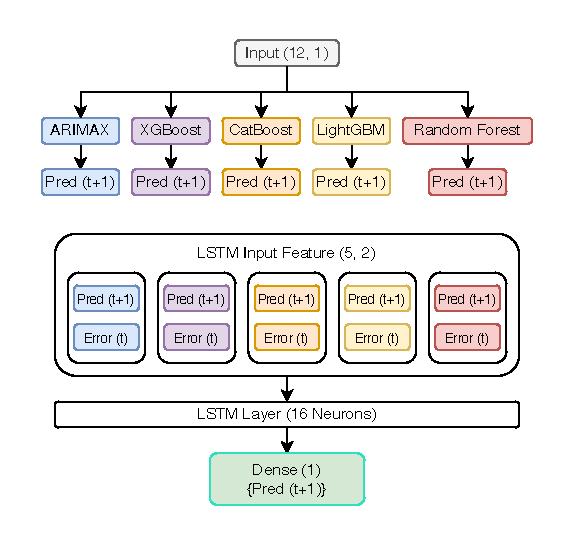
\includegraphics[width=\textwidth]{Images/Ensemble_.pdf}
    \caption{Custom Ensemble Learning Architecture}
    \label{fig:custom_ensemble_architecture}
\end{figure}

The ensemble leverages the strengths of both:
\begin{itemize}
    \item \textit{Tree-based models} for capturing nonlinear patterns.
    \item \textit{ARIMAX} for linear autoregressive temporal relationships.
    \item \textit{LSTM} for modeling sequential dependence in prediction errors and combining predictions dynamically.
\end{itemize}

\subsection{Meta Feature Representation}

Each input $\mathbf{x}_t \in \mathbb{R}^{d}$ is passed to the base models and ARIMAX to produce scalar predictions $\hat{y}_{t}^{(i)}$ for each model $i$. Along with each prediction, a rolling MAE score is computed:

\begin{equation}
\text{MAE}_{t}^{(i)} = \frac{1}{w} \sum_{j=t-w+1}^{t} \left| y_j - \hat{y}_j^{(i)} \right|
\end{equation}

The meta input $\mathbf{z}_t \in \mathbb{R}^{5 \times 2}$ at time $t$ is constructed as:

\begin{equation}
\mathbf{z}_t = \left[ \left( \hat{y}_t^{(i)}, \text{MAE}_t^{(i)} \right) \right]_{i=1}^5
\end{equation}

where $i = \{ \text{XGB, LGB, CAT, RF, ARIMAX} \}$.

\subsection{MetaLearner Model}

The MetaLearner is a neural network consisting of:
\begin{itemize}
    \item \textbf{Input:} Sequence of shape $(5, 2)$
    \item \textbf{LSTM Layer:} 16 units with ReLU activation
    \item \textbf{Dense Output Layer:} Single scalar prediction
\end{itemize}

The output of the MetaLearner is given by:

\begin{equation}
\hat{y}_t^{\text{meta}} = \text{Dense} \left( \text{LSTM}(\mathbf{z}_t) \right)
\end{equation}

\subsection{Algorithm Flow}

\begin{enumerate}
    \item \textbf{Load and Split Dataset} into train, validation, and test sets.
    \item \textbf{Train Base Models:}
    \begin{itemize}
        \item XGBoost
        \item LightGBM
        \item CatBoost
        \item RandomForest
        \item ARIMAX (on training set)
    \end{itemize}
    \item \textbf{Generate Meta Features:}
    \begin{itemize}
        \item For each time step in train/val/test:
        \begin{itemize}
            \item Predict using each base model
            \item Forecast ARIMAX
            \item Calculate rolling MAE of each model
            \item Store $(\text{prediction}, \text{MAE})$ as meta feature
        \end{itemize}
    \end{itemize}
    \item \textbf{Train MetaLearner (LSTM):}
    \begin{itemize}
        \item Input: meta feature sequence $(5, 2)$
        \item Output: predicted value $\hat{y}_t$
    \end{itemize}
    \item \textbf{Evaluate on Validation and Test Set} using RMSE
\end{enumerate}

% \subsection{Pseudocode}

% \begin{verbatim}
% Function CustomEnsembleLearningModel(X_train, y_train, X_val, y_val, X_test, y_test):
%     Step 1: Train base models (XGB, LGB, CAT, RF)
%     Step 2: Fit ARIMAX on y_train with X_train as exog
%     Step 3: For each sample in train/val/test:
%         - Predict using all base models
%         - Forecast ARIMAX
%         - Compute rolling MAE for each model
%         - Store [prediction, MAE] as meta feature
%     Step 4: Stack meta features into 3D array of shape (N, 5, 2)
%     Step 5: Build and train LSTM model on meta features
%     Step 6: Predict on validation and test meta features
%     Step 7: Compute and log RMSE for all models and MetaNet

% End Function
% \end{verbatim}
\section{Transformer-based GAN Architecture}

In this section, we propose a sequence-to-one forecasting framework inspired by the TTS-GAN architecture as proposed in \cite{yoon_time-series_2019}. The model consists of a Generator and a Discriminator, both built using Transformer Encoder blocks to effectively process multivariate sequential data. The architecture leverages self-attention mechanisms to capture temporal dependencies and contextual relationships across multiple input features.

The Generator takes a fixed-length historical input sequence and outputs a single predicted return value for the next time step. The Discriminator, in turn, distinguishes between the real future value and the one generated by the Generator, thereby adversarially training the system to enhance the quality and realism of predictions.

This Transformer-based GAN approach enables more robust modeling of complex nonlinear patterns in financial time series data and shows promise in generating plausible and sharp return estimates for short-term stock price prediction.

\subsection{Generator Architecture}

The Generator $G$ takes as input a multivariate sequence $X \in \mathbb{R}^{T \times d}$ of length $T=60$ with $d=12$ features and predicts a scalar output $\hat{y}_{t+1} \in \mathbb{R}$. The input is first linearly projected into an embedding space and combined with learned positional encodings:
\[
x'_t = \text{Dense}(X_t) + \text{Embedding}(t)
\]
This representation is passed through $L$ stacked Transformer Encoder blocks, followed by a Global Average Pooling operation and a final dense layer:
\[
\hat{y}_{t+1} = G(X) = \text{Dense}(\text{GAP}(\text{TransformerBlocks}(x')))
\]

\subsection{Discriminator Architecture}

The Discriminator $D$ takes as input a univariate sequence of length 61: a real or generated scalar return $\hat{y}_{t+1}$ appended to the past 60 true values $y_{t-59}, \dots, y_t$. The architecture is similar to the Generator: a dense projection followed by positional embeddings and multiple Transformer blocks. The final output is a scalar in $[0, 1]$:
\[
D(Z) = \sigma(\text{Dense}(\text{GAP}(\text{TransformerBlocks}(Z))))
\]
where $Z \in \mathbb{R}^{61 \times 1}$ is the sequence and $\sigma$ denotes the sigmoid activation.

\begin{figure}[h!]
    \centering
    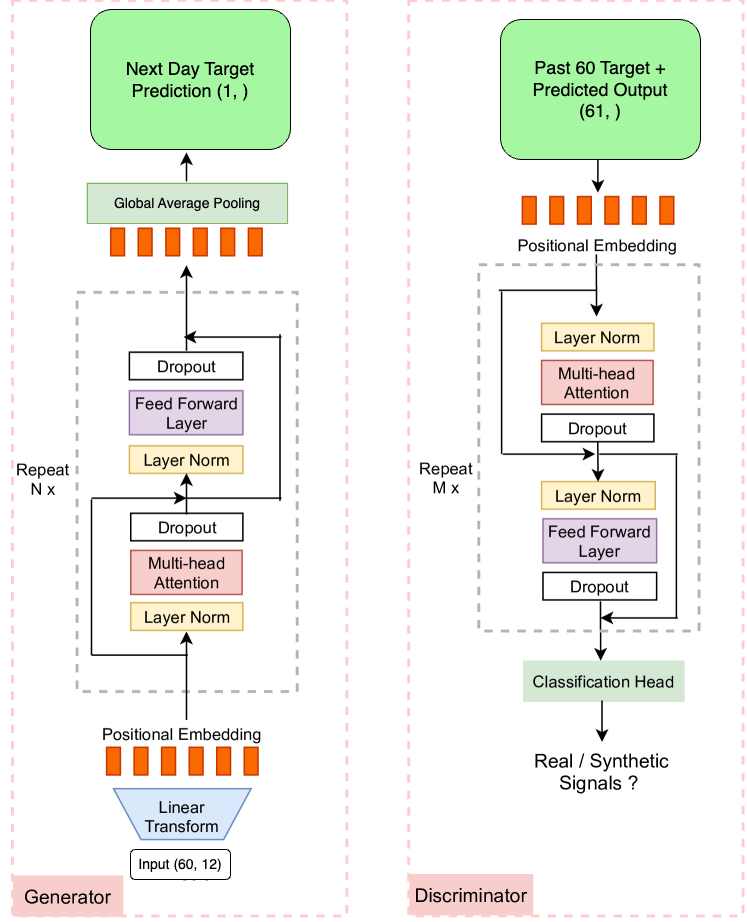
\includegraphics[width=\textwidth]{Images/TimeGAN.png}
    \caption{Transformer-based GAN architecture showing the structure of the Generator and Discriminator.}
    \label{fig:transformer_gan_architecture}
\end{figure}

\subsection{Transformer Encoder Block}

\begingroup
\sloppy
Each Transformer Encoder block consists of a Multi-Head Self-Attention (MHSA) layer followed by a feed-forward network (FFN):
\endgroup

\[
\text{MHSA}(X) = \text{LayerNorm}(X + \text{Dropout}(\text{MultiHeadAttention}(X, X)))
\]
\[
\text{FFN}(X) = \text{LayerNorm}(\text{MHSA}(X) + \text{Dropout}(\text{Dense}(\text{GELU}(\text{Dense}(X)))))
\]

\subsection{Training Procedure}

The model is trained using a combination of mean squared error (MSE) and adversarial loss. Let $y_{t+1}$ be the true target and $\hat{y}_{t+1}$ the generator's prediction. The Discriminator loss is given by:
\[
\mathcal{L}_D = \text{BCE}(1, D(y_{\text{seq}}^{\text{real}})) + \text{BCE}(0, D(y_{\text{seq}}^{\text{fake}}))
\]
where $y_{\text{seq}}^{\text{real}} = [y_{t-59}, \dots, y_t, y_{t+1}]$ and $y_{\text{seq}}^{\text{fake}} = [y_{t-59}, \dots, y_t, \hat{y}_{t+1}]$.

The Generator is optimized using:
\[
\mathcal{L}_G = \text{MSE}(y_{t+1}, \hat{y}_{t+1}) + \lambda \cdot \text{BCE}(1, D(y_{\text{seq}}^{\text{fake}}))
\]
where $\lambda$ is a small weighting factor for adversarial loss (e.g., $\lambda = 0.01$).

\subsection{Optimization}

Gradients are computed using backpropagation through both the Generator and Discriminator. Separate optimizers are used for $G$ and $D$, and their parameters are updated iteratively at each training step.

% \newpage
\section{RAGIC Architecture for Financial Time Series Forecasting}

\subsection{Overview}

The \textbf{RAGIC (Risk-Aware Generator with Integrated Critic)} architecture is a hybrid deep learning framework developed to model financial time series data with enhanced robustness and generalization. It integrates noise-injected attention mechanisms, temporal modeling using multi-head attention and TCNs, and adversarial learning using a Wasserstein critic to improve prediction performance on volatile data.

RAGIC is designed to forecast the next value in a sequence (e.g., stock return or price) by conditioning on multivariate historical data. It consists of three main modules:
\begin{itemize}
    \item \textbf{Risk Module} (attention + noise for uncertainty modeling)
    \item \textbf{Temporal Module} (Transformer + TCN for time series understanding)
    \item \textbf{Critic} (Wasserstein GAN discriminator to enforce realistic prediction quality)
\end{itemize}

\begin{figure}[H]
    \centering
    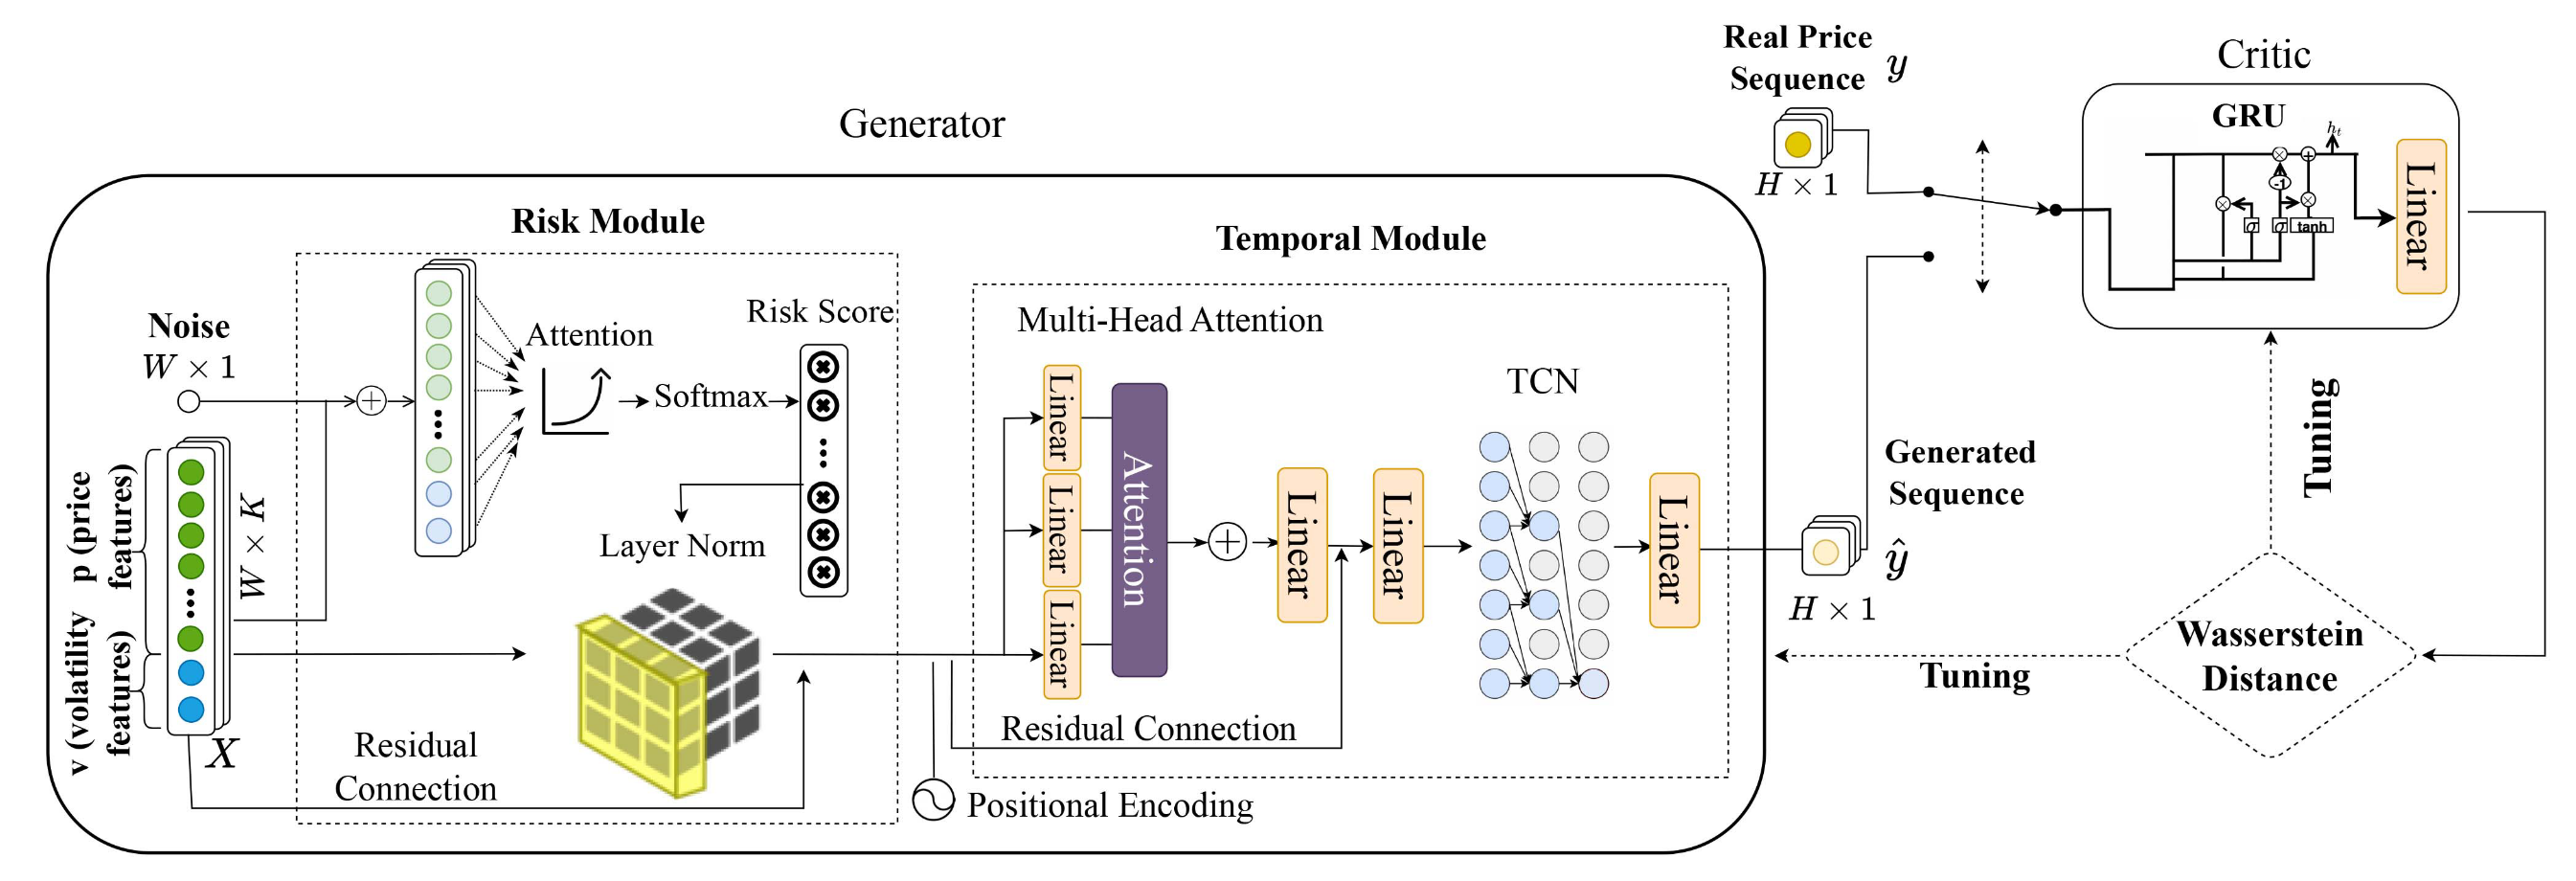
\includegraphics[width=0.95\textwidth]{Images/Screenshot 2025-05-19 at 15.00.48.png}
    \caption{RAGIC Architecture diagram \cite{gu_ragic_2025}.}
    \label{fig:ragic_architecture}
\end{figure}
The overall architecture of RAGIC, including its three key modules and data flow, is illustrated in Figure~\ref{fig:ragic_architecture}.

\subsection{Theory and Components}

\subsubsection{Risk Module}

The \textbf{Risk Module} aims to model market uncertainty by injecting Gaussian noise into the input sequence and applying attention-based weighting. This mechanism allows the model to focus on uncertain and potentially volatile patterns.

Given input $X \in \mathbb{R}^{W \times K}$ and noise $\epsilon \sim \mathcal{N}(0, I)$ of shape $\mathbb{R}^{W \times 1}$, the steps are:
\begin{enumerate}
    \item Concatenate: $X_{\text{aug}} = [X \, | \, \epsilon]$
    \item Attention weights: $a = \text{softmax}(WX_{\text{aug}})$
    \item Weighted input: $\tilde{X} = a \odot X$
    \item Residual connection and normalization: $X_{\text{risk}} = \text{LayerNorm}(\tilde{X} + X)$
\end{enumerate}

\subsubsection{Temporal Module}

The \textbf{Temporal Module} processes the output of the risk module through a combination of positional embeddings, multi-head self-attention, and a two-layer Temporal Convolutional Network (TCN). It captures both long-term dependencies and local temporal dynamics.

Let $X_{\text{risk}} \in \mathbb{R}^{W \times K}$ be the input:
\begin{enumerate}
    \item Add positional embedding: $X_{\text{pos}} = X_{\text{risk}} + \text{Embed}(\text{position})$
    \item Multi-head attention: $X_{\text{attn}} = \text{MultiHeadAttention}(X_{\text{pos}})$
    \item Residual + LayerNorm: $X_{\text{norm}} = \text{LayerNorm}(X_{\text{attn}} + X_{\text{pos}})$
    \item TCN: Two dilated Conv1D layers with causal padding and ReLU activation.
    \item Global pooling and dense output: $\hat{y} = \text{Dense}( \text{GlobalAvgPool}(X_{\text{tcn}}) )$
\end{enumerate}

\subsubsection{Generator and Critic}

\textbf{Generator:} Composed of the Risk and Temporal modules, it predicts the next time-step value $\hat{y}$ from a sequence $X$ and random noise $\epsilon$.

\textbf{Critic:} A GRU-based Wasserstein discriminator that receives a full sequence of $W$ time steps (including either the predicted or real value as the last step) and outputs a scalar "realness" score:
\[
D(X) = \text{Dense}(\text{GRU}(X))
\]

\subsection{Training Algorithm}

The RAGIC framework is trained in an adversarial manner, where the Generator aims to produce realistic predictions, and the Critic learns to distinguish between real and generated sequences. The loss functions are:

\begin{itemize}
    \item \textbf{Generator Loss (Predictor):}
    \[
    \mathcal{L}_G = \text{MSE}(y, \hat{y})
    \]
    
    \item \textbf{Critic Loss:}
    \[
    \mathcal{L}_D = \mathbb{E}_{\text{fake}}[D(X_{\text{fake}})] - \mathbb{E}_{\text{real}}[D(X_{\text{real}})]
    \]
\end{itemize}

\subsection{Workflow}

\begin{enumerate}
    \item Load time series data $X \in \mathbb{R}^{T \times K}$ and target $Y \in \mathbb{R}^T$.
    \item Create overlapping sequences of length $W=60$.
    \item Split into training and test sets.
    \item For each epoch:
    \begin{itemize}
        \item Generate noise $\epsilon$ for each batch.
        \item \textbf{Train Generator:}
            \begin{itemize}
                \item Pass $X$ and $\epsilon$ through Risk $\rightarrow$ Temporal to get $\hat{y}$.
                \item Minimize MSE with ground truth $y$.
            \end{itemize}
        \item \textbf{Train Critic:}
            \begin{itemize}
                \item Concatenate predicted or real $y$ with $X[:, 1:, :]$ to form fake/real sequences.
                \item Maximize $\mathcal{L}_D$ (Wasserstein loss).
            \end{itemize}
    \end{itemize}
    \item Track losses and visualize performance.
\end{enumerate}

\subsection{Applications}

The RAGIC architecture is designed for time series forecasting tasks with inherent uncertainty and noise, such as:
\begin{itemize}
    \item Stock return forecasting
    \item Volatility prediction
    \item Economic indicator forecasting
\end{itemize}

Its integration of noise-aware attention and adversarial learning enables better modeling of complex financial dynamics.


\chapter{Results and Evaluation}

\section{Evaluation Metrics and Criteria}

\subsection*{Root Mean Squared Error (RMSE)}
The Root Mean Squared Error (RMSE) is a criterion used to evaluate the accuracy of the model’s forecast. It is calculated as the square root of the arithmetic mean of the squared differences between actual and predicted values. RMSE provides insights into the scale of errors, especially for regression models. It is defined as:

\begin{equation}
\text{RMSE} = \sqrt{\frac{1}{n} \sum_{i=1}^{n} (y_i - \hat{y}_i)^2}
\end{equation}

where:
\begin{itemize}
    \item \( n \): Number of observations
    \item \( y_i \): Actual value of the \(i^{th}\) observation
    \item \( \hat{y}_i \): Predicted value of the \(i^{th}\) observation
\end{itemize}

\subsection*{R-squared (R²)}
The coefficient of determination, \(R^2\), measures the proportion of variance in the dependent variable explained by the model. Its range is from 0 to 1, where 1 indicates that the model explains all the variation, and 0 indicates no explanatory power. It is defined as:

\begin{equation}
R^2 = 1 - \frac{\sum_{i=1}^{n} (y_i - \hat{y}_i)^2}{\sum_{i=1}^{n} (y_i - \bar{y})^2}
\end{equation}

where:
\begin{itemize}
    \item \( n \): Number of observations
    \item \( y_i \): True value of the \(i^{th}\) observation
    \item \( \hat{y}_i \): Predicted value of the \(i^{th}\) observation
    \item \( \bar{y} \): Mean of the actual values
\end{itemize}

\section{Performance of Enhanced Hybrid LSTM-RLS Architecture}

\subsection{Results Before and After Shift Adjustment}

\begin{figure}[h!]
    \centering
    \includegraphics[width=\textwidth]{Images/ActvsPred.pdf}
    \caption{Original vs. Predicted Stock Prices}
    \label{fig:refinedApproachRes1}
\end{figure}

\begin{figure}[h!]
    \centering
    \includegraphics[width=\textwidth]{Images/returns_comparision.pdf}
    \caption{Returns: Original vs. Predicted Prices}
    \label{fig:refinedApproachRes2}
\end{figure}

\begin{table}[h!]
\centering
\caption{LSTM-RLS Performance Metrics}
\begin{tabular}{|l|c|c|c|}
\hline
\textbf{LSTM-RLS}  & \textbf{Daily Returns} & \textbf{Weekly Returns} & \textbf{Daily Close} \\ \hline
\textbf{RMSE}      & 0.76\%                 & 1.44\%                 & 161.8935             \\ \hline
\textbf{R2}        & -0.0636                & -0.038                 & 0.9956               \\ \hline
\end{tabular}

\label{tab:lstm_rls_performance}
\end{table}

\begin{figure}[h!]
    \centering
    \includegraphics[width=\textwidth]{Images/ActvsPredshift.pdf}
    \caption{Stock Prices: Shifted Predictions (-1)}
    \label{fig:revisedApproachshift1}
\end{figure}

\begin{table}[h!]
\centering
\caption{RMSE Comparison for Daily Returns (LSTM-RLS)}
\begin{tabular}{|l|c|}
\hline
\multicolumn{2}{|c|}{\textbf{LSTM-RLS Error between Actual and Predicted Daily Returns}} \\ \hline
\textbf{Original RMSE}       & 1.01\%   \\ \hline
\textbf{RMSE with Shift - 1} & \textbf{0.24\%} \\ \hline
\end{tabular}

\label{tab:lstm_rls_shift}
\end{table}

\subsection{Performance with Multi-Feature Dataset}

\begin{figure}[h!]
    \centering
    \includegraphics[width=\textwidth]{Images/5_ActvsPred_LSTM_RLS.pdf}
    \caption{Stock Prices: Actual vs. Predicted Daily Returns}
    \label{fig:actvspred_returns}
\end{figure}

\begin{table}[h!]
\centering
\caption{Performance Metrics for Multi-Feature LSTM-RLS}
\label{tab:performance_metrics}
\begin{tabular}{|l|c|}
\hline
\textbf{Metric}   & \textbf{Value}  \\ \hline
RMSE              & 0.91\%  \\ \hline
R\textsuperscript{2} Score & -0.061  \\ \hline
\end{tabular}
\end{table}

\section{Performance of DNS Architecture}

Figure~\ref{fig:DNSplot} shows the best actual vs predicted plot when trained and tested on the DNS architecture to remove lag in prediction.

% Modify figure sizes according to your needs
\begin{figure}[h!]
    \centering
    \includegraphics[width=\textwidth]{Images/actual_vs_predicted_main_N2_50seq_LSTM.pdf}
    \caption{ Comparison of Stock Prices and Returns (Shifted -1)}
    \label{fig:DNSplot}
\end{figure}

Table~\ref{tab:DNSres} shows the RMSE and R2 results for the DNS architecture with all combination of networks used.

\begin{table}[ht]
\centering
\caption{Comparison of DNS Models: LSTM-SDM, LSTM-MA, RBF-SDM, and RBF-MA}
\begin{tabular}{|l|c|c|c|c|}
\hline
\textbf{DNS}     & \textbf{LSTM-SDM} & \textbf{LSTM-MA} & \textbf{RBF-SDM} & \textbf{RBF-MA} \\ \hline
\textbf{RMSE}    & 1082.0187          & 688.529          & \textbf{328.7387}         & 479.8617        \\ \hline
\textbf{R2}      & 0.8092             & 0.9227           & \textbf{0.9823}  & 0.9624          \\ \hline
\end{tabular}

\label{tab:DNSres}
\end{table}

\newpage
\section{ARIMA-LSTM Residual Framework Results}

\subsection{ARIMAX Test Predictions}
Figures~\ref{fig:arimax_close} and \ref{fig:arimax_returns} present the test predictions from the ARIMAX model when the output variable is close price and daily returns, respectively.

\begin{figure}[h!]
    \centering
    \includegraphics[width=\textwidth]{Images/3_final_predictions_close.pdf}
    \caption{ARIMAX Test Predictions - Output: Close Price}
    \label{fig:arimax_close}
\end{figure}

\begin{figure}[h!]
    \centering
    \includegraphics[width=\textwidth]{Images/3_final_predictions_return.pdf}
    \caption{ARIMAX Test Predictions - Output: Returns}
    \label{fig:arimax_returns}
\end{figure}

\subsection{Final Test Predictions}
Figures~\ref{fig:final_close} and \ref{fig:final_returns} illustrate the final test predictions after integrating LSTM when the output is close price and daily returns.

\begin{figure}[h!]
    \centering
    \includegraphics[width=\textwidth]{Images/3_final_predictions_close.pdf}
    \caption{Final Test Predictions - Output: Close Price}
    \label{fig:final_close}
\end{figure}

\begin{figure}[h!]
    \centering
    \includegraphics[width=\textwidth]{Images/3_final_predictions_return.pdf}
    \caption{Final Test Predictions - Output: Returns}
    \label{fig:final_returns}
\end{figure}

\subsection{Performance Metrics}
Table~\ref{tab:performance_arimax_final} compares the test RMSE and \( R^2 \) scores for ARIMAX and the final model when predicting close prices and daily returns.

\begin{table}[h!]
\centering
\caption{Test RMSE and \( R^2 \) Score for ARIMAX and Final Model}
\label{tab:performance_arimax_final}
\begin{tabular}{|l|c|c|}
\hline
\textbf{Model} & \textbf{RMSE} & \textbf{\( R^2 \) Score} \\ \hline
ARIMAX (Close) & 7431.43 & -35.47 \\ \hline
ARIMAX (Returns) & 0.703\% & 0.36 \\ \hline
Final Model (Close) & 7394.61 & -35.11 \\ \hline
Final Model (Returns) & 0.669\% & 0.42 \\ \hline
\end{tabular}
\end{table}

\subsection{Impact of RLS on Final Predictions}

\begin{figure}[h!]
    \centering
    \includegraphics[width=\textwidth]{Images/6_Final_Pred.pdf}
    \caption{Actual vs. Predicted Returns After Applying RLS to Final Predictions}
    \label{fig:rls_on_residuals}
\end{figure}

\begin{table}[h!]
\centering
\caption{Performance Metrics After Applying RLS to Residuals}
\label{tab:rls_residuals_performance}
\begin{tabular}{|l|c|}
\hline
\textbf{Metric}   & \textbf{Value}  \\ \hline
RMSE              & 0.72\%  \\ \hline
R\textsuperscript{2} Score & 0.32  \\ \hline
\end{tabular}
\end{table}

\section{Multi-Feature LSTM Results}
This section presents the evaluation results of the Multi-Feature LSTM Forecasting Framework, focusing on its performance in predicting daily close returns. The evaluation metrics and visualizations demonstrate the accuracy and adaptability of the framework, as well as its ability to handle real-time updates as per the incremental training methodology discussed earlier.

\subsection{Evaluation Metrics and Analysis}
The framework's performance is evaluated using two key visualizations:
\begin{enumerate}
    \item \textbf{Absolute Error vs Total RMSE:} Figure~\ref{fig:absolute_error_rmse} plots the absolute error between actual and predicted daily close returns in one time step prediction. Besides, it plots the total RMSE of the test set for the entire duration of evaluation. This graph plots how well the architecture minimizes the errors from predictions.

    \item \textbf{Actual vs Predicted Close Returns:} Figure~\ref{fig:actual_vs_predicted} depicts the agreement
Between actual and predicted daily close returns with re-training of the model after every prediction following incremental training approach. The above plot indicates the learning ability of the model as well as real-time predictive accuracy.
\end{enumerate}

\subsection{Interpretation of Results}
\begin{itemize}
    \item The high absolute error values observed in Figure~\ref{fig:absolute_error_rmse} verify that the model is not very good at predicting daily close returns.
    \item The difference between the actual and predicted returns in  Figure~\ref{fig:actual_vs_predicted} is a result of how the incremental training works, allowing the model to capture recent market trends.
    \item A comparison of absolute error with total RMSE clearly highlights the significance of one-time step prediction error minimization for successful application in algorithmic trading.
\end{itemize}

\subsection{Visualization of Results}
The plots illustrating the framework's performance are provided below:

\begin{figure}[h!]
    \centering
    \includegraphics[width=\textwidth]{Images/absolute_error_vs_rmse.pdf}
    \caption{Absolute error between actual and predicted one-time step daily close return, compared with the total RMSE of the test data.}
    \label{fig:absolute_error_rmse}
\end{figure}

\begin{figure}[h!]
    \centering
    \includegraphics[width=\textwidth]{Images/actual_vs_predicted_returns.pdf}
    \caption{Actual vs Predicted daily close return where the model is retrained after each prediction as per the incremental training methodology.}
    \label{fig:actual_vs_predicted}
\end{figure}

\newpage
\section{GARCH Model Results}

\subsection{Evaluation Metrics and Performance}

Both the ARIMAX and GARCHX models were trained on the same return-based dataset to separately model the conditional mean and variance components of the time series. While the ARIMAX model produced valid forecasts, the GARCHX model failed to detect meaningful volatility patterns in the residuals and generated nearly constant predictions, with changes appearing only after the fifth decimal place. As a result, the GARCHX predictions were almost indistinguishable from a flat line, indicating its inability to model residual volatility in this dataset.

\subsection{Residuals from ARIMAX Predictions}

To analyze the deviations captured by the GARCH model, we plot the residuals obtained by subtracting ARIMAX predictions from the actual values.

\begin{figure}[h!]
    \centering
    \includegraphics[width=\textwidth]{Images/7_Residuals.pdf}
    \caption{Residuals: Actual Values - ARIMAX Predictions}
    \label{fig:residuals_actual_arimax}
\end{figure}

\subsection{Combined ARIMAX + GARCHX Predictions}

\begin{figure}[h!]
    \centering
    \includegraphics[width=\textwidth]{Images/7_garchx_arimax.pdf}
    \caption{Actual vs. Predicted Returns Using ARIMAX + GARCHX}
    \label{fig:garch_actual_pred}
\end{figure}

\begin{table}[h!]
\centering
\caption{Performance Metrics of ARIMAX + GARCHX Model}
\label{tab:arimax_garch_performance}
\begin{tabular}{|l|c|}
\hline
\textbf{Metric}   & \textbf{Value}  \\ \hline
RMSE              & 0.703\%  \\ \hline
R\textsuperscript{2} Score & 0.36  \\ \hline
\end{tabular}
\end{table}

\subsection{GARCHX-Only Predictions}

To further evaluate the GARCHX model, we isolate and plot its predicted volatility component (added to ARIMAX residuals). As seen below, these predictions are nearly flat, reflecting the model's inability to detect or amplify residual variations.

\begin{figure}[h!]
    \centering
    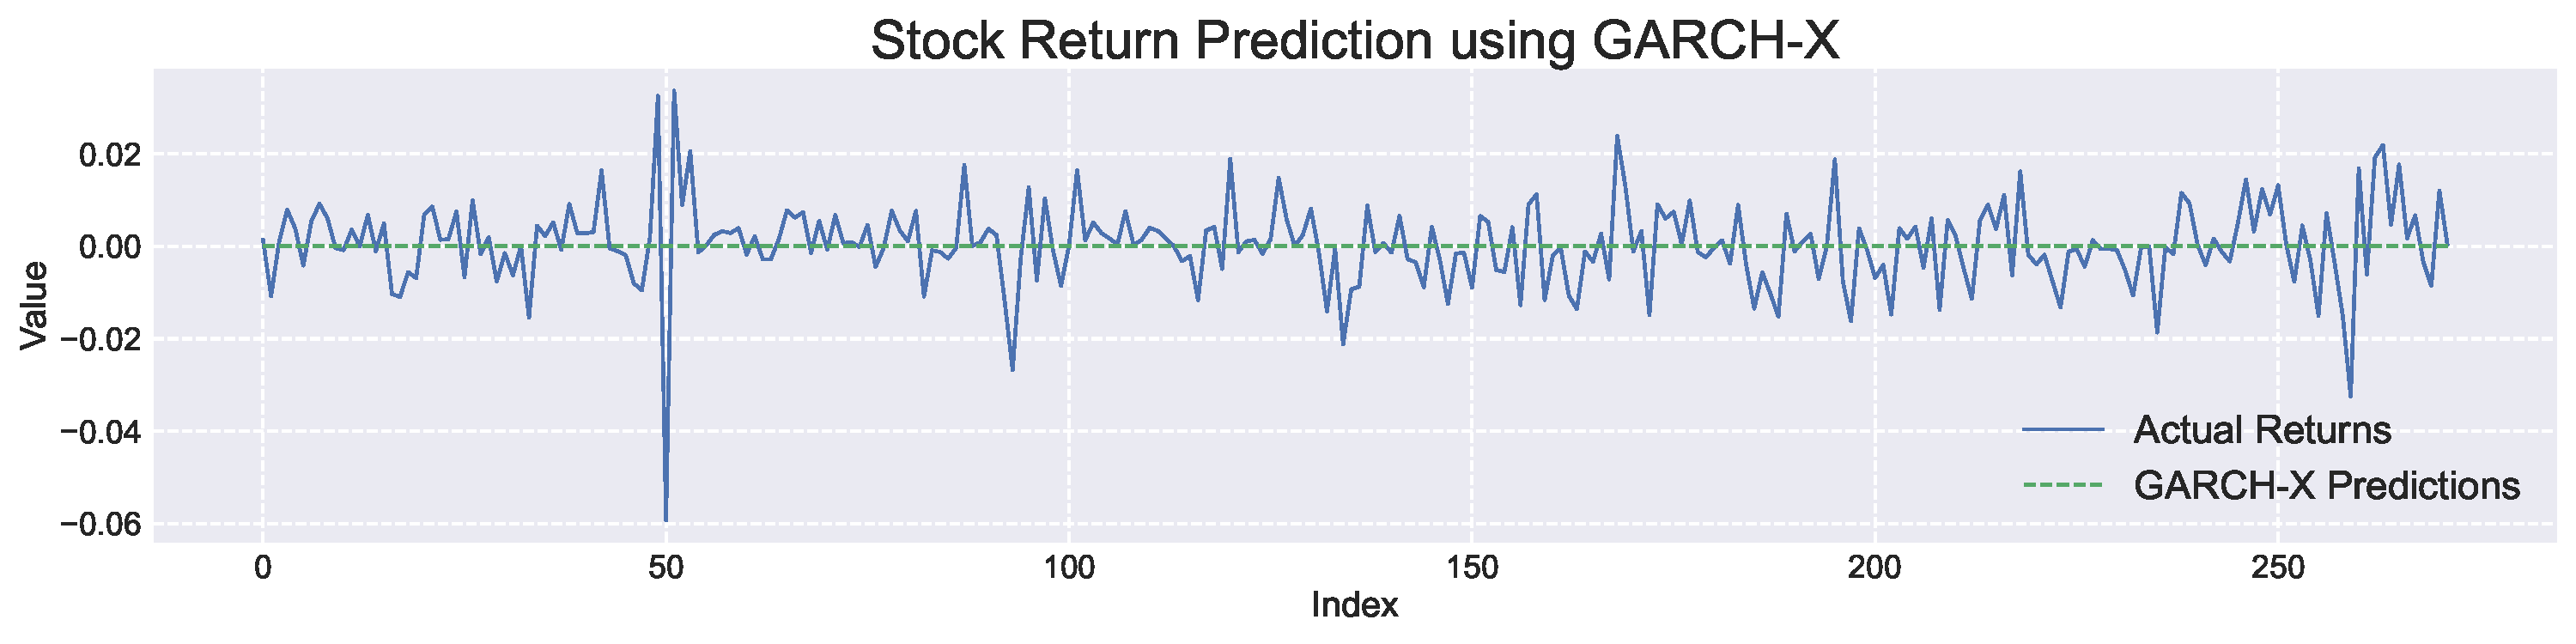
\includegraphics[width=\textwidth]{Images/7_garchx.pdf}
    \caption{Predicted Residuals from GARCHX Model}
    \label{fig:garchx_only_pred}
\end{figure}

\begin{table}[h!]
\centering
\caption{Performance Metrics of GARCHX-Only Predictions}
\label{tab:garchx_only_performance}
\begin{tabular}{|l|c|}
\hline
\textbf{Metric}   & \textbf{Value}  \\ \hline
RMSE              & 0.9219\%  \\ \hline
R\textsuperscript{2} Score & -0.001381  \\ \hline
\end{tabular}
\end{table}

% \newpage
\section{Stochastic Volatility Results}
\subsection{Actual vs Predicted Returns}
Figure~\ref{fig:sv_actual_vs_pred} shows the normalized actual returns plotted against the normalized filtered log-volatility estimates from the stochastic volatility model.

\subsection{Distribution Comparison}
Figure~\ref{fig:sv_density} displays the kernel density estimation (KDE) curves of actual returns versus fitted returns from the stochastic volatility model, highlighting how well the model captures the return distribution characteristics.

\subsection{Performance Metrics}
\begin{itemize}
    \item \textbf{RMSE:} 0.0104
    \item \textbf{R\textsuperscript{2} Score:} -0.2091
\end{itemize}

\begin{figure}[h!]
    \centering
    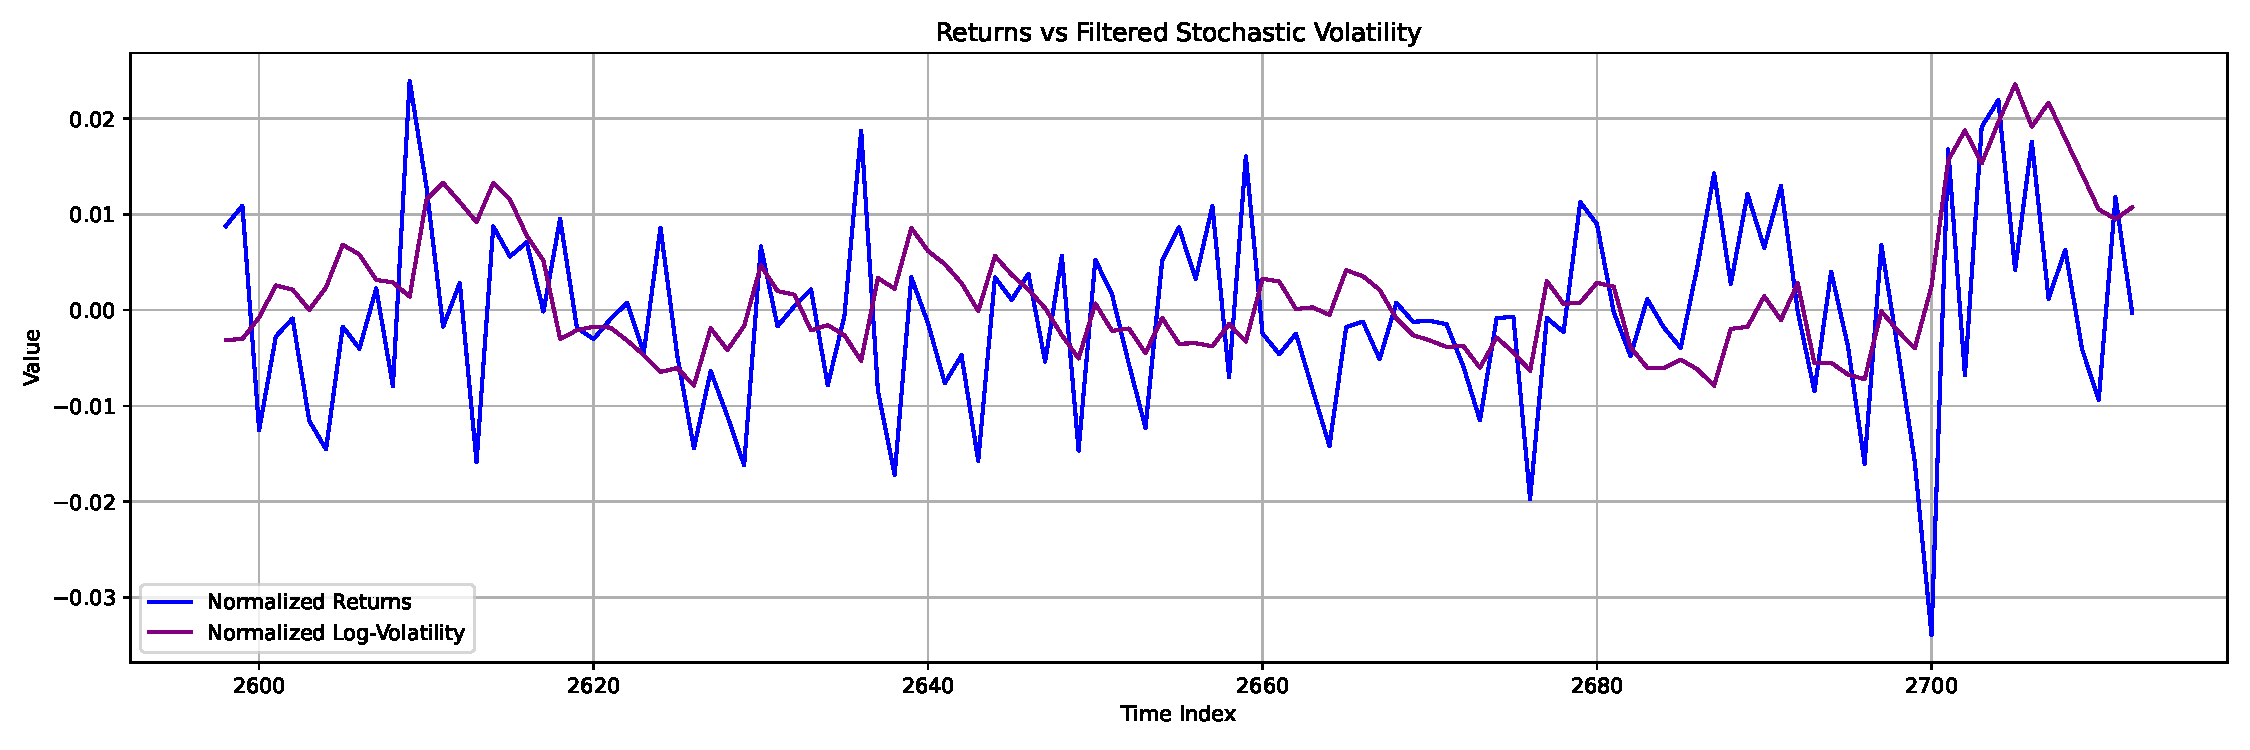
\includegraphics[width=\textwidth]{Images/stochastic_volatility.pdf}
    \caption{Normalized actual returns vs filtered log-volatility (Stochastic Volatility Model).}
    \label{fig:sv_actual_vs_pred}
\end{figure}

\begin{figure}[h!]
    \centering
    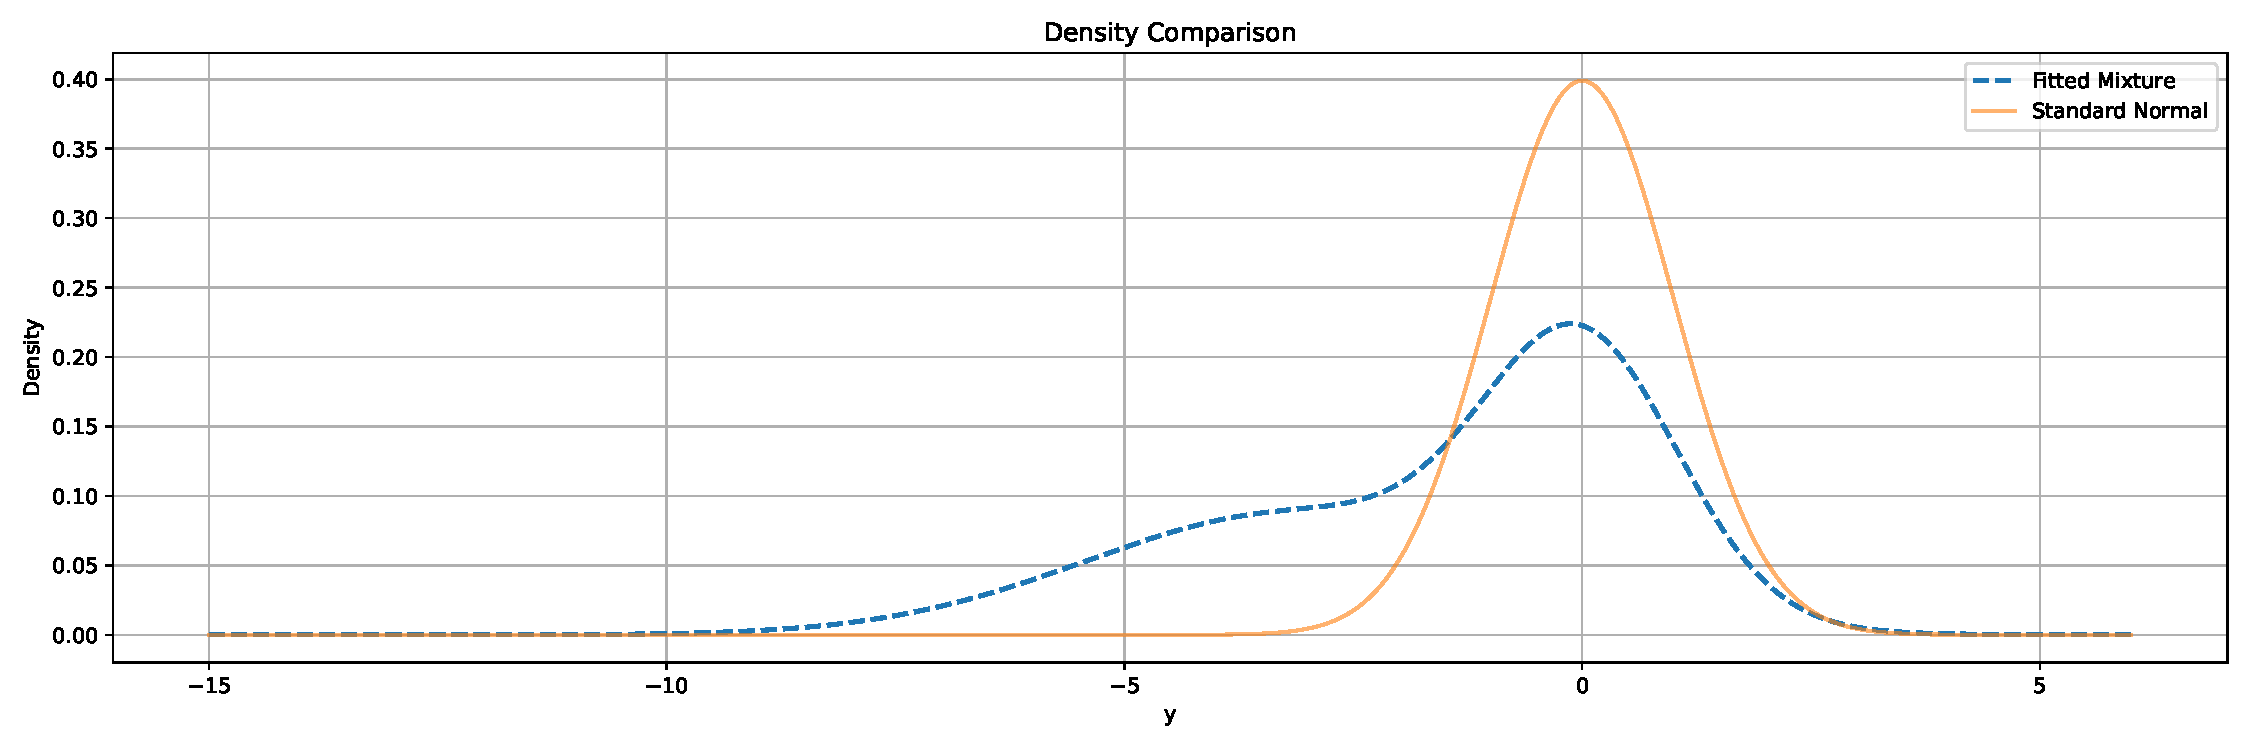
\includegraphics[width=\textwidth]{Images/stochastic_volatility_density.pdf}
    \caption{Density comparison of actual returns vs fitted returns (Stochastic Volatility Model).}
    \label{fig:sv_density}
\end{figure}

\section{Ensemble Learning Results}

\subsection{Actual vs Predicted Returns}
Figure~\ref{fig:ensemble_actual_vs_pred} presents the predicted daily returns from the ensemble meta-learner compared with the actual close returns.

\subsection{Performance Metrics}
\begin{itemize}
    \item \textbf{MetaNet RMSE (Validation):} 0.0065
    \item \textbf{MetaNet RMSE (Test):} 0.0064
    \item \textbf{MetaNet R\textsuperscript{2} Score (Test):} 0.5130
\end{itemize}

\subsection{Base Model Comparison}
Table~\ref{tab:ensemble_base_models} shows the RMSE values for each base model on both the validation and test sets, highlighting the performance of MetaNet as the final predictor.

\begin{table}[h!]
\centering
\caption{RMSE of Base Models and MetaNet (Validation and Test Sets)}
\label{tab:ensemble_base_models}
\begin{tabular}{lcc}
\toprule
\textbf{Model} & \textbf{RMSE (Validation)} & \textbf{RMSE (Test)} \\
\midrule
XGBoost     & 0.00670 & 0.00624 \\
LightGBM    & 0.00670 & 0.00638 \\
CatBoost    & 0.00663 & 0.00636 \\
RandomForest & 0.00667 & 0.00658 \\
ARIMAX      & 0.00713 & 0.00766 \\
MetaNet     & \textbf{0.00655} & \textbf{0.00638} \\
\bottomrule
\end{tabular}
\end{table}

\begin{figure}[h!]
    \centering
    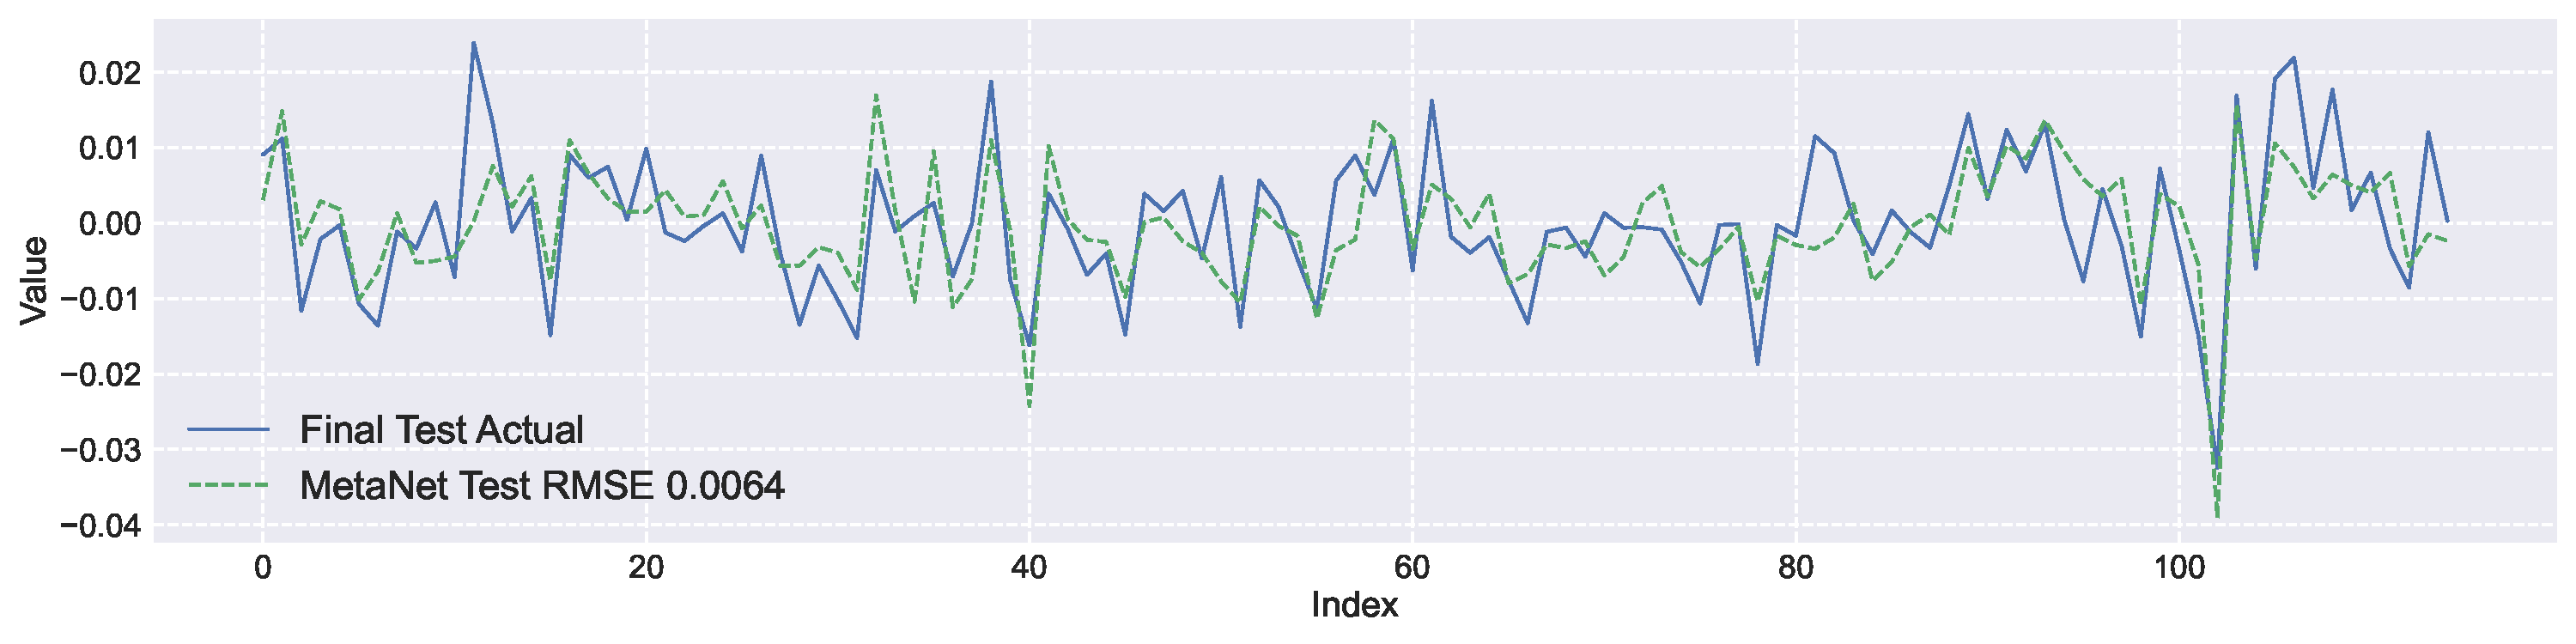
\includegraphics[width=\textwidth]{Images/metanet_final_test_plot__1.pdf}
    \caption{Actual vs Predicted daily close return (Ensemble Meta-Learner).}
    \label{fig:ensemble_actual_vs_pred}
\end{figure}

\section{Transformer GAN Results}
\subsection{Actual vs Predicted Returns}
Figure~\ref{fig:tgan_actual_vs_pred} illustrates the ability of the Transformer-based GAN to replicate daily return dynamics.

\begin{figure}[h!]
    \centering
    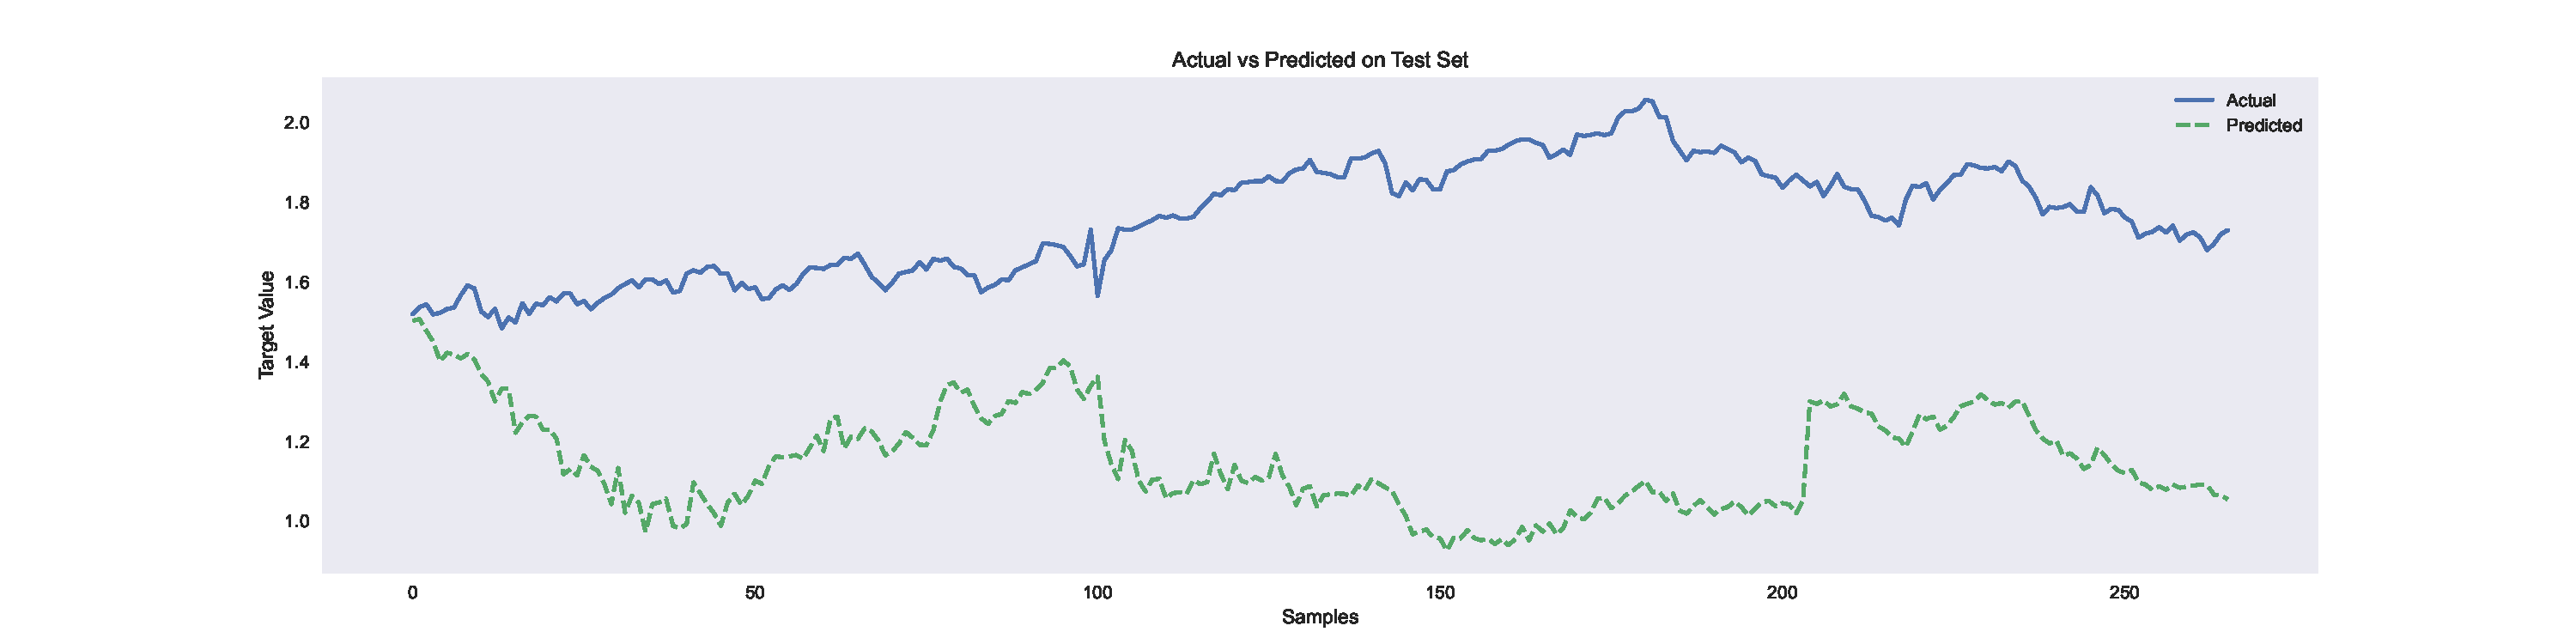
\includegraphics[width=\textwidth]{Images/_8_ActualVsPred_c.pdf}
    \caption{Actual vs Predicted daily close return (Transformer GAN).}
    \label{fig:tgan_actual_vs_pred}
\end{figure}

\noindent The Transformer GAN demonstrates poor predictive capability, with predictions deviating significantly from actual return values and exhibiting erratic behavior. Quantitative evaluation confirms this outcome, with a high RMSE of \textcolor{red}{14550.0515} and a highly negative \( R^2 \) score of \textcolor{red}{-12.2655}, indicating that the model performs substantially worse than a simple mean-based prediction.

\newpage
\section{RAGIC Framework Results}
\subsection{Actual vs Predicted Returns}
Figure~\ref{fig:ragic_actual_vs_pred} compares the predicted returns from the RAGIC framework against the actual returns, reflecting the model’s interpretability and precision.

\begin{figure}[h!]
    \centering
    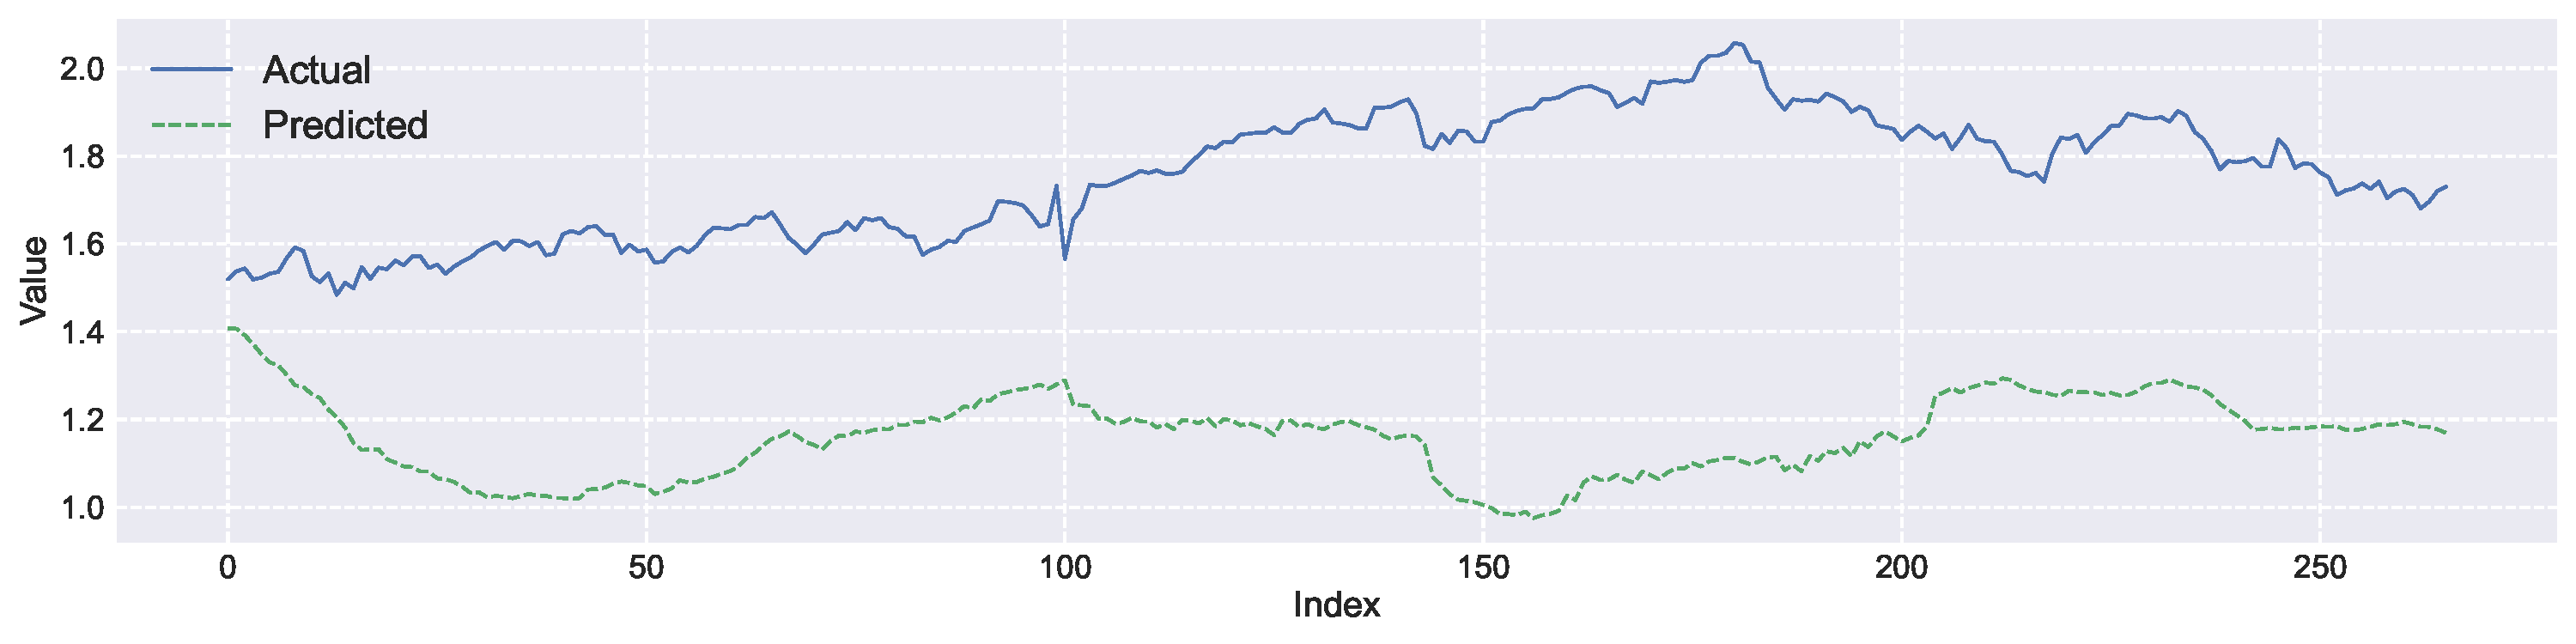
\includegraphics[width=\textwidth]{Images/9_Act_vs_Pred_Point.pdf}
    \caption{Actual vs Predicted daily close return (RAGIC Framework).}
    \label{fig:ragic_actual_vs_pred}
\end{figure}

\noindent Despite the use of an attention-based risk module and temporal modeling in the RAGIC framework, the predictions diverge drastically from the actual values. This is quantitatively supported by an RMSE of \textcolor{red}{16192.9227} and an extremely negative \( R^2 \) score of \textcolor{red}{-37.1641}, indicating the model fails to capture any meaningful signal from the data and performs far worse than baseline methods.

\section{Results Comparison}

\begin{table}[h!]
    \centering
    \caption{Comparison of All Model Performances}
    \label{tab:all_model_comparison}
    \begin{tabular}{|l|c|c|}
    \hline
    \textbf{Model (Target)} & \textbf{RMSE} & \textbf{R\textsuperscript{2} Score} \\ \hline
    
    LSTM-RLS (Daily Returns) & \textcolor{red}{0.76\%} & \textcolor{red}{-0.0636} \\ \hline
    LSTM-RLS (Weekly Returns) & \textcolor{red}{1.44\%} & \textcolor{red}{-0.038} \\ \hline
    LSTM-RLS (Daily Close) & 161.8935 & 0.9956 \\ \hline
    LSTM-RLS, Manually Shifted (Returns) & 0.24\% & 0.9982 \\ \hline
    LSTM-RLS, Multi-Feature Input (Returns) & \textcolor{red}{0.91\%} & \textcolor{red}{-0.061} \\ \hline
    
    DNS - LSTM-SDM (Close) & 1082.0187 & 0.8092 \\ \hline
    DNS - LSTM-MA (Close) & 688.529 & 0.9227 \\ \hline
    DNS - RBF-SDM (Close) & 328.7387 & 0.9823 \\ \hline
    DNS - RBF-MA (Close) & 479.8617 & 0.9624 \\ \hline
    
    ARIMAX (Close) & \textcolor{red}{7431.43} & \textcolor{red}{-35.47} \\ \hline
    ARIMAX-LSTM (Returns) & 0.703\% & 0.36 \\ \hline
    ARIMAX Model + RLS (Returns) & 0.72\% & 0.32 \\ \hline
    
    Multi-Feature LSTM (Returns) & \textcolor{red}{0.9072\%} & \textcolor{red}{-0.01376} \\ \hline
    GARCH Model (Returns) & \textcolor{red}{0.9219\%} & \textcolor{red}{-0.001381} \\ \hline
    Stochastic Volatility Model (Returns) & \textcolor{red}{1.04\%} & \textcolor{red}{-0.2091} \\ \hline
    Ensemble Learning Model (Returns) & \textbf{0.638\%} & \textbf{0.5130} \\ \hline
    Transformer GAN (Close) & \textcolor{red}{14550.0515} & \textcolor{red}{-12.2655} \\ \hline
    RAGIC Architecture (Close) & \textcolor{red}{16192.9227} & \textcolor{red}{-37.1641} \\ \hline
    
    \end{tabular}
\end{table}

\noindent As seen in Table~\ref{tab:all_model_comparison}, the \textbf{Ensemble Learning Model} achieves the lowest RMSE of \textbf{0.638\%}, demonstrating the highest predictive accuracy among all evaluated models. The \textbf{LSTM-RLS (Daily Close)} model also performs exceptionally well with an R\textsuperscript{2} score of 0.9956, highlighting its effectiveness in modeling price levels. In contrast, traditional models like \textbf{ARIMAX (Close)} suffer from high error and a significantly negative R\textsuperscript{2} score. Models such as the \textbf{Multi-Feature LSTM}, \textbf{GARCH Model}, and \textbf{Stochastic Volatility Model} yield relatively poor results, with RMSE values close to or above 0.9\% and negative R\textsuperscript{2} scores. Traditional approaches like \textbf{ARIMAX (Close)} and even advanced generative models such as \textbf{Transformer GAN} and the \textbf{RAGIC Architecture} perform poorly, showing extremely high RMSEs and strongly negative R\textsuperscript{2} values. Hybrid models like the \textbf{DNS} and \textbf{LSTM-RLS} variants generally outperform classical approaches, especially in denoised trend and price-based forecasting.

\chapter{Discussions and Challenges}

\section{Key Findings}
Although the RMSE and \( R^2 \) score of the enhanced hybrid LSTM-RLS model were lower, the actual vs. prediction plot revealed a constant lag of one time step in the predicted stock prices. To address this issue, the DNS architecture was adopted. However, despite experimenting with various combinations of activation functions and slope trend methods, the model could not eliminate the lag.

Consequently, the DNS architecture was replaced by the ARIMA-LSTM Residual Integration Framework. Since ARIMA did not perform as expected in predicting the linear component, LSTM was utilized to predict both linear and non-linear components. However, this model also failed to remove the lag and exhibited a higher RMSE compared to other model architectures.

To further enhance performance, additional features were incorporated, and a dataset with multiple features was developed as described earlier. The Multi-Feature LSTM Forecasting Framework was then employed. Despite these enhancements, this model architecture, when combined with the proposed training method, was also unable to eliminate the lag in predictions.

Additionally, the Hybrid LSTM-RLS with a multi-feature input did not perform well. The reason behind this is that the LSTM output, which consists of daily returns, is highly volatile in nature, making it difficult for the model to generalize effectively.

The ARIMAX-LSTM-RLS model also slightly reduced performance, suggesting that the final predictions obtained from the residuals architecture do not serve as suitable inputs for the RLS model in an online prediction setting.

Furthermore, GARCH, for some reason, failed to capture any volatility (variance) in the residuals obtained after the mean predictions by ARIMAX. As a result, the final predictions produced by GARCH were identical to those obtained from ARIMAX alone, rendering GARCH ineffective in improving prediction performance.

Based on the comparative performance of different architectures tested in this dissertation, the residuals architecture has demonstrated the best predictive capability so far.

In the case of the Stochastic Volatility model, although lags were observed at certain points, the filtered volatility estimates closely followed the overall return patterns with moderate error, demonstrating the model's ability to track dynamic volatility behavior.

For the Ensemble Learning Framework, predictions from ARIMAX, Random Forest, CatBoost, LightGBM, and XGBoost were combined using an LSTM-based MetaNet. This approach successfully eliminated the one-time step lag and closely followed the actual return patterns. However, occasional directional mispredictions led to slightly elevated RMSE values. Despite this, the ensemble method outperformed all other architectures tested in this study.

The Transformer GAN-based architecture and the RAGIC model, implemented directly as described in their respective papers, showed significantly higher prediction errors. Even after extended training (up to 500 epochs), both architectures struggled to generalize. Due to limited time, these GAN-based models were not significantly modified, which might have contributed to their underperformance.

To conclude, among all the tested models and algorithms, the Ensemble Learning Framework delivered the best overall performance in terms of pattern tracking, lag elimination, and balanced error metrics.
\section{Challenges and Model Refinement}
A significant challenge faced during the development of the hybrid models was the persistent lag in long-term predictions. Despite repeated efforts to refine the models—particularly the hybrid LSTM-RLS architectures—the lag in predictions continued to appear consistently. While the introduction of alternative models aimed at mitigating this lag did result in lower RMSE values in some cases, the core issue of delayed predictions remained unresolved.

This underscores the difficulty in simultaneously achieving high accuracy and eliminating temporal lag, especially in sequential financial data. The lag persisted even with models explicitly designed for short-term responsiveness, highlighting a fundamental trade-off between complexity and real-time adaptability.

Volatility modeling through GARCH also posed substantial challenges. Despite being a well-established method, GARCH failed to capture any meaningful variance in the ARIMAX residuals. The model consistently predicted near-zero volatility, rendering it ineffective in enhancing the prediction accuracy. This unexpected outcome underlines the limitations of applying classical volatility models to highly noisy and non-linear residual structures in financial time series.

The Stochastic Volatility framework, although able to capture the broad shape and dynamics of volatility, occasionally exhibited lag and divergence from actual return magnitudes. This suggests that while it is effective in estimating underlying variance trends, aligning those estimates with return dynamics remains a complex task.

Ensemble Learning, though the most successful overall, brought its own set of challenges. Integrating predictions from multiple diverse models—including ARIMAX, Random Forest, CatBoost, LightGBM, and XGBoost—into a MetaNet required careful feature normalization, input alignment, and consistent retraining to ensure stability. Additionally, occasional directional mispredictions contributed to local spikes in error despite the overall reduction in lag.

Implementation of Transformer GAN and RAGIC architectures also presented technical and methodological difficulties. Due to time constraints, these models were implemented with minimal modifications to their original architectures. Despite extensive training, they showed high prediction errors and poor generalization. The complexity of GAN training and sensitivity to hyperparameter tuning further limited their effectiveness in this study.

In summary, while significant advancements were made in predictive modeling of stock returns, persistent challenges such as time-step lag, ineffective volatility modeling, and difficulties in training generative architectures remain unresolved. These limitations highlight areas for future research, particularly in adaptive modeling, robust volatility estimation, and customized GAN architectures for financial time series forecasting.
\chapter{Conclusion and Future Direction}

\section{Conclusion}
This work explored multiple hybrid and deep learning-based models to improve stock return prediction. The initial Hybrid LSTM-RLS model showed consistent one-step lag, which persisted across the DNS and ARIMA-LSTM Residual Integration frameworks, despite minor RMSE improvements. The Multi-Feature LSTM Framework improved input representation but failed to resolve the lag issue.

GARCH integration over ARIMAX residuals proved ineffective, consistently predicting near-zero volatility. The Stochastic Volatility model followed general return patterns but exhibited lags and deviations. Transformer GAN and RAGIC architectures, implemented with minimal tuning, resulted in high prediction errors.

The Ensemble Learning Framework, combining ARIMAX, tree-based models, and a MetaNet, delivered the best performance by eliminating lag and closely tracking return trends, despite some directional prediction errors. Overall, ensemble learning proved the most effective strategy for real-time stock return forecasting among all models tested.

\section{Future Direction}
Future work will focus on refining the RAGIC and Transformer GAN architectures, as well as exploring alternative GAN-based frameworks aimed at achieving lag-less and low-loss stock return predictions. Additionally, incorporating more sophisticated feature engineering and advanced model tuning strategies could further enhance prediction accuracy and address the remaining challenges identified in this study.


\chapter{Publications}

\section*{Publications Based on This Dissertation}

\begin{itemize}
    \item Dr. Jigarkumar Shah, Dr. Bhubon Chandra Mech, Parth Sharma, \textit{“Hybrid Approaches for Improving Stock Price Forecasting Using Co-Integration of LSTM Network and RLS Algorithm”}, \textbf{28th Nirma International Conference on Management (NICOM 2025)}, held from \textbf{January 8 to January 10, 2025}. The presentation was part of the sub-theme \textbf{Finance and Accounting}, under the track titled “\textit{Financial Technologies and Digitalization: Financial Analytics and Machine Learning \& Deep Learning Applications in Finance.}”
\end{itemize}

\section*{Publications under Other Guides}

\begin{itemize}
    \item Parth Sharma, Rajesh Kumar Mohapatra, Dev Patel, Ritesh Vyas, Santosh Satapathy, \textit{“Automated Classification of EEG Patterns from BrainEEG Signals for Predicting Sleep Deficiency”}, \textbf{5th International Conference on Machine Learning, IoT and Big Data (ICMIB 2025)}, held from \textbf{April 4 to April 6, 2025}, Pandit Deendayal Energy University, Gandhinagar, Gujarat.
\end{itemize}

\section*{Target Journals for Future Publication}

Based on the research conducted in this dissertation, the following journals have been identified as suitable targets for future publication:

\section*{1. The Journal of Finance and Data Science}
\begin{itemize}
    \item \textbf{Impact Factor:} 3.9
    \item \textbf{Scopus Indexed:} Yes
\end{itemize}

\section*{2. Data Science in Finance and Economics}
\begin{itemize}
    \item \textbf{Impact Factor:} 1.3
    \item \textbf{Scopus Indexed:} No
\end{itemize}

These journals have been selected based on their relevance to the subject areas of finance, time series forecasting, and data science.

\clearpage
\addcontentsline{toc}{chapter}{Bibliography}
\printbibliography

\end{document}